% !TEX encoding = UTF-8
% !TEX TS-program = pdflatex
% !TEX root = tesi.tex
% !TEX spellcheck = it-IT

% PDF/A filecontents
\RequirePackage{filecontents}
\begin{filecontents*}{\jobname.xmpdata}
  \Title{Document’s title}
  \Author{Author’s name}
  \Language{it-IT}
  \Subject{The abstract, or short description.}
  \Keywords{keyword1\sep keyword2\sep keyword3}
\end{filecontents*}

\documentclass[10pt,                    % corpo del font principale
               a4paper,                 % carta A4
               twoside,                 % impagina per fronte-retro
               openright,               % inizio capitoli a destra
               english,
               italian,
               ]{book}

%**************************************************************
% Importazione package
%**************************************************************

\PassOptionsToPackage{dvipsnames}{xcolor} % colori PDF/A

\usepackage{colorprofiles}
\usepackage{multirow}

\usepackage[a-2b,mathxmp]{pdfx}[2018/12/22]
                                        % configurazione PDF/A
                                        % validare in https://www.pdf-online.com/osa/validate.aspx

%\usepackage{amsmath,amssymb,amsthm}    % matematica

\usepackage[T1]{fontenc}                % codifica dei font:
                                        % NOTA BENE! richiede una distribuzione *completa* di LaTeX

\usepackage[utf8]{inputenc}             % codifica di input; anche [latin1] va bene
                                        % NOTA BENE! va accordata con le preferenze dell'editor

\usepackage[english, italian]{babel}    % per scrivere in italiano e in inglese;
                                        % l'ultima lingua (l'italiano) risulta predefinita

\usepackage{bookmark}                   % segnalibri

\usepackage{caption}                    % didascalie

\usepackage{chngpage,calc}              % centra il frontespizio

\usepackage{csquotes}                   % gestisce automaticamente i caratteri (")

\usepackage{emptypage}                  % pagine vuote senza testatina e piede di pagina

\usepackage{epigraph}			% per epigrafi

\usepackage{eurosym}                    % simbolo dell'euro

%\usepackage{indentfirst}               % rientra il primo paragrafo di ogni sezione

\usepackage{graphicx}                   % immagini

\usepackage{hyperref}                   % collegamenti ipertestuali

\usepackage[binding=5mm]{layaureo}      % margini ottimizzati per l'A4; rilegatura di 5 mm

\usepackage{listings}                   % codici

\usepackage{microtype}                  % microtipografia

\usepackage{mparhack,fixltx2e,relsize}  % finezze tipografiche

\usepackage{nameref}                    % visualizza nome dei riferimenti
\usepackage[font=small]{quoting}        % citazioni

\usepackage{subfig}                     % sottofigure, sottotabelle

\usepackage[italian]{varioref}          % riferimenti completi della pagina

\usepackage{booktabs}                   % tabelle
\usepackage{tabularx}                   % tabelle di larghezza prefissata
\usepackage{longtable}                  % tabelle su più pagine
\usepackage{ltxtable}                   % tabelle su più pagine e adattabili in larghezza

\usepackage[toc, acronym]{glossaries}   % glossario
                                        % per includerlo nel documento bisogna:
                                        % 1. compilare una prima volta tesi.tex;
                                        % 2. eseguire: makeindex -s tesi.ist -t tesi.glg -o tesi.gls tesi.glo
                                        % 3. eseguire: makeindex -s tesi.ist -t tesi.alg -o tesi.acr tesi.acn
                                        % 4. compilare due volte tesi.tex.

\usepackage[backend=biber,style=verbose-ibid,hyperref,backref]{biblatex}
                                        % eccellente pacchetto per la bibliografia;
                                        % produce uno stile di citazione autore-anno;
                                        % lo stile "numeric-comp" produce riferimenti numerici
                                        % per includerlo nel documento bisogna:
                                        % 1. compilare una prima volta tesi.tex;
                                        % 2. eseguire: biber tesi
                                        % 3. compilare ancora tesi.tex.


\renewcommand\tabularxcolumn[1]{m{#1}}% for vertical centering text in X column

%**************************************************************
% file contenente le impostazioni della tesi
%**************************************************************

%**************************************************************
% Frontespizio
%**************************************************************

% Autore
\newcommand{\myName}{Enrico Buratto}
\newcommand{\myTitle}{Migrazione a dispositivo mobile di una applicazione web tramite tecnologia Ionic}

% Tipo di tesi
\newcommand{\myDegree}{Tesi di laurea}

% Università
\newcommand{\myUni}{Università degli Studi di Padova}

% Facoltà
\newcommand{\myFaculty}{Corso di Laurea in Informatica}

% Dipartimento
\newcommand{\myDepartment}{Dipartimento di Matematica "Tullio Levi-Civita"}

% Titolo del relatore
\newcommand{\profTitle}{Prof.}

% Relatore
\newcommand{\myProf}{Tullio Vardanega}

% Luogo
\newcommand{\myLocation}{Padova}

% Anno accademico
\newcommand{\myAA}{2019-2020}

% Data discussione
\newcommand{\myTime}{Dicembre 2020}


%**************************************************************
% Impostazioni di impaginazione
% see: http://wwwcdf.pd.infn.it/AppuntiLinux/a2547.htm
%**************************************************************

\setlength{\parindent}{14pt}   % larghezza rientro della prima riga
\setlength{\parskip}{0pt}   % distanza tra i paragrafi


%**************************************************************
% Impostazioni di biblatex
%**************************************************************
\bibliography{bibliografia} % database di biblatex

\defbibheading{bibliography} {
    \cleardoublepage
    \phantomsection
    \addcontentsline{toc}{chapter}{\bibname}
    \chapter*{\bibname\markboth{\bibname}{\bibname}}
}

\setlength\bibitemsep{1.5\itemsep} % spazio tra entry

\DeclareBibliographyCategory{opere}
\DeclareBibliographyCategory{web}

\addtocategory{opere}{womak:lean-thinking}
\addtocategory{web}{site:agile-manifesto}

\defbibheading{opere}{\section*{Riferimenti bibliografici}}
\defbibheading{web}{\section*{Siti Web consultati}}


%**************************************************************
% Impostazioni di caption
%**************************************************************
\captionsetup{
    tableposition=top,
    figureposition=bottom,
    font=small,
    format=hang,
    labelfont=bf
}

%**************************************************************
% Impostazioni di glossaries
%**************************************************************

%**************************************************************
% Acronimi
%**************************************************************
\renewcommand{\acronymname}{Acronimi e abbreviazioni}

\newacronym[description={\glslink{apig}{Application Program Interface}}]
    {api}{API}{Application Program Interface}

\newacronym[description={\glslink{umlg}{Unified Modeling Language}}]
    {uml}{UML}{Unified Modeling Language}

%**************************************************************
% Glossario
%**************************************************************
%\renewcommand{\glossaryname}{Glossario}

% \newglossaryentry{apig}
% {
%     name=\glslink{api}{API},
%     text=Application Program Interface,
%     sort=api,
%     description={in informatica con il termine \emph{Application Programming Interface API} (ing. interfaccia di programmazione di un'applicazione) si indica ogni insieme di procedure disponibili al programmatore, di solito raggruppate a formare un set di strumenti specifici per l'espletamento di un determinato compito all'interno di un certo programma. La finalità è ottenere un'astrazione, di solito tra l'hardware e il programmatore o tra software a basso e quello ad alto livello semplificando così il lavoro di programmazione}
% }
%
% \newglossaryentry{umlg}
% {
%     name=\glslink{uml}{UML},
%     text=UML,
%     sort=uml,
%     description={in ingegneria del software \emph{UML, Unified Modeling Language} (ing. linguaggio di modellazione unificato) è un linguaggio di modellazione e specifica basato sul paradigma object-oriented. L'\emph{UML} svolge un'importantissima funzione di ``lingua franca'' nella comunità della progettazione e programmazione a oggetti. Gran parte della letteratura di settore usa tale linguaggio per descrivere soluzioni analitiche e progettuali in modo sintetico e comprensibile a un vasto pubblico}
% }
 % database di termini
\makeglossaries


%**************************************************************
% Impostazioni di graphicx
%**************************************************************
\graphicspath{{immagini/}} % cartella dove sono riposte le immagini


%**************************************************************
% Impostazioni di hyperref
%**************************************************************
\hypersetup{
    %hyperfootnotes=false,
    %pdfpagelabels,
    %draft,	% = elimina tutti i link (utile per stampe in bianco e nero)
    colorlinks=true,
    linktocpage=true,
    pdfstartpage=1,
    pdfstartview=,
    % decommenta la riga seguente per avere link in nero (per esempio per la stampa in bianco e nero)
    %colorlinks=false, linktocpage=false, pdfborder={0 0 0}, pdfstartpage=1, pdfstartview=FitV,
    breaklinks=true,
    pdfpagemode=UseNone,
    pageanchor=true,
    pdfpagemode=UseOutlines,
    plainpages=false,
    bookmarksnumbered,
    bookmarksopen=true,
    bookmarksopenlevel=1,
    hypertexnames=true,
    pdfhighlight=/O,
    %nesting=true,
    %frenchlinks,
    urlcolor=webbrown,
    linkcolor=RoyalBlue,
    citecolor=webgreen,
    %pagecolor=RoyalBlue,
    %urlcolor=Black, linkcolor=Black, citecolor=Black, %pagecolor=Black,
    pdftitle={\myTitle},
    pdfauthor={\textcopyright\ \myName, \myUni, \myFaculty},
    pdfsubject={},
    pdfkeywords={},
    pdfcreator={pdfLaTeX},
    pdfproducer={LaTeX}
}

%**************************************************************
% Impostazioni di itemize
%**************************************************************
%\renewcommand{\labelitemi}{$\ast$}

\renewcommand{\labelitemi}{$\bullet$}
%\renewcommand{\labelitemii}{$\cdot$}
%\renewcommand{\labelitemiii}{$\diamond$}
%\renewcommand{\labelitemiv}{$\ast$}


%**************************************************************
% Impostazioni di listings
%**************************************************************
\lstset{
    language=[LaTeX]Tex,%C++,
    keywordstyle=\color{RoyalBlue}, %\bfseries,
    basicstyle=\small\ttfamily,
    %identifierstyle=\color{NavyBlue},
    commentstyle=\color{Green}\ttfamily,
    stringstyle=\rmfamily,
    numbers=none, %left,%
    numberstyle=\scriptsize, %\tiny
    stepnumber=5,
    numbersep=8pt,
    showstringspaces=false,
    breaklines=true,
    frameround=ftff,
    frame=single
}


%**************************************************************
% Impostazioni di xcolor
%**************************************************************
\definecolor{webgreen}{rgb}{0,.5,0}
\definecolor{webbrown}{rgb}{.6,0,0}


%**************************************************************
% Altro
%**************************************************************

\newcommand{\omissis}{[\dots\negthinspace]} % produce [...]

% eccezioni all'algoritmo di sillabazione
\hyphenation
{
    ma-cro-istru-zio-ne
    gi-ral-din
}

\newcommand{\sectionname}{sezione}
\addto\captionsitalian{\renewcommand{\figurename}{Figura}
                       \renewcommand{\tablename}{Tabella}}

\newcommand{\glsfirstoccur}{\ap{{[g]}}}

\newcommand{\intro}[1]{\emph{\textsf{#1}}}

%**************************************************************
% Environment per ``rischi''
%**************************************************************
\newcounter{riskcounter}                % define a counter
\setcounter{riskcounter}{0}             % set the counter to some initial value

%%%% Parameters
% #1: Title
\newenvironment{risk}[1]{
    \refstepcounter{riskcounter}        % increment counter
    \par \noindent                      % start new paragraph
    \textbf{\arabic{riskcounter}. #1}   % display the title before the
                                        % content of the environment is displayed
}{
    \par\medskip
}

\newcommand{\riskname}{Rischio}

\newcommand{\riskdescription}[1]{\textbf{\\Descrizione:} #1.}

\newcommand{\risksolution}[1]{\textbf{\\Soluzione:} #1.}

%**************************************************************
% Environment per ``use case''
%**************************************************************
\newcounter{usecasecounter}             % define a counter
\setcounter{usecasecounter}{0}          % set the counter to some initial value

%%%% Parameters
% #1: ID
% #2: Nome
\newenvironment{usecase}[2]{
    \renewcommand{\theusecasecounter}{\usecasename #1}  % this is where the display of
                                                        % the counter is overwritten/modified
    \refstepcounter{usecasecounter}             % increment counter
    \vspace{10pt}
    \par \noindent                              % start new paragraph
    {\large \textbf{\usecasename #1: #2}}       % display the title before the
                                                % content of the environment is displayed
    \medskip
}{
    \medskip
}

\newcommand{\usecasename}{UC}

\newcommand{\usecaseactors}[1]{\textbf{\\Attori Principali:} #1. \vspace{4pt}}
\newcommand{\usecasepre}[1]{\textbf{\\Precondizioni:} #1. \vspace{4pt}}
\newcommand{\usecasedesc}[1]{\textbf{\\Descrizione:} #1. \vspace{4pt}}
\newcommand{\usecasepost}[1]{\textbf{\\Postcondizioni:} #1. \vspace{4pt}}
\newcommand{\usecasealt}[1]{\textbf{\\Scenario Alternativo:} #1. \vspace{4pt}}

%**************************************************************
% Environment per ``namespace description''
%**************************************************************

\newenvironment{namespacedesc}{
    \vspace{10pt}
    \par \noindent                              % start new paragraph
    \begin{description}
}{
    \end{description}
    \medskip
}

\newcommand{\classdesc}[2]{\item[\textbf{#1:}] #2}
                     % file con le impostazioni personali

\begin{document}
%**************************************************************
% Materiale iniziale
%**************************************************************
\frontmatter
% !TEX encoding = UTF-8
% !TEX TS-program = pdflatex
% !TEX root = ../tesi.tex

%**************************************************************
% Frontespizio 
%**************************************************************
\begin{titlepage}

\begin{center}

\begin{LARGE}
\textbf{\myUni}\\
\end{LARGE}

\vspace{10pt}

\begin{Large}
\textsc{\myDepartment}\\
\end{Large}

\vspace{10pt}

\begin{large}
\textsc{\myFaculty}\\
\end{large}

\vspace{30pt}
\begin{figure}[htbp]
\begin{center}

\includegraphics[height=6cm]{logo-unipd}
\end{center}
\end{figure}
\vspace{30pt} 

\begin{LARGE}
\begin{center}
\textbf{\myTitle}\\
\end{center}
\end{LARGE}

\vspace{10pt} 

\begin{large}
\textsl{\myDegree}\\
\end{large}

\vspace{40pt} 

\begin{large}
\begin{flushleft}
\textit{Relatore}\\ 
\vspace{5pt} 
\profTitle \myProf
\end{flushleft}

\vspace{0pt} 

\begin{flushright}
\textit{Laureando}\\ 
\vspace{5pt} 
\myName
\end{flushright}
\end{large}

\vspace{40pt}

\line(1, 0){338} \\
\begin{normalsize}
\textsc{Anno Accademico \myAA}
\end{normalsize}

\end{center}
\end{titlepage} 
% !TEX encoding = UTF-8
% !TEX TS-program = pdflatex
% !TEX root = ../tesi.tex

%**************************************************************
% Colophon
%**************************************************************
\clearpage
\phantomsection
\thispagestyle{empty}

\hfill

\vfill

\noindent\myName: \textit{\myTitle,}
\myDegree,
\textcopyright\ \myTime.
% % !TEX encoding = UTF-8
% !TEX TS-program = pdflatex
% !TEX root = ../tesi.tex

%**************************************************************
% Dedica
%**************************************************************
\cleardoublepage
\phantomsection
\thispagestyle{empty}
\pdfbookmark{Dedica}{Dedica}

\vspace*{3cm}

\begin{center}
% Qua dentro mettere la citazione. \\ \medskip
% --- Persona Citata
\end{center}

\medskip

\begin{center}
% Qua dentro mettere dedica
\end{center}

% !TEX encoding = UTF-8
% !TEX TS-program = pdflatex
% !TEX root = ../tesi.tex

%**************************************************************
% Sommario
%**************************************************************
\cleardoublepage
\phantomsection
\pdfbookmark{Sommario}{Sommario}
\begingroup
\let\clearpage\relax
\let\cleardoublepage\relax
\let\cleardoublepage\relax

\chapter*{Sommario}

Il seguente documento descrive il tirocinio che ho svolto presso la sede di Padova dell'azienda \textbf{Sync Lab s.r.l.}, d'ora in poi \textit{"Sync Lab"} o \textit{"l'azienda"}, nel periodo che va dal 31/08/2020 al 23/10/2020. Lo stage ha avuto una durata complessiva di circa \textbf{300 ore}, ed è stato supervisionato dal mio tutor esterno, Andrea Giunta, e dal mio relatore, prof. Tullio Vardanega.\\
Scopo dello stage è stato studiare e utilizzare il \textit{framework Ionic}, tecnologia che permette la realizzazione di applicazioni \textit{mobile} ibride a partire da codice \textit{JavaScript} o \textit{TypeScript}, per il \textbf{\textit{porting}} di un applicativo web preesistente su dispositivi mobili. \\
La migrazione verso dispositivi mobili che ho effettuato si è basata sulla componente \textit{front-end} dell'applicativo \textit{SyncTrace}, sviluppata da altri studenti durante i precedenti tirocini e completata ufficialmente il 28/08/2020; questa componente è stata sviluppata tramite il \textit{framework Angular} in accoppiata al linguaggio \textit{TypeScript}. \\
L'\textbf{obiettivo} di questo applicativo è inquadrabile nell'ambito del \textit{contact tracing} per la prevenzione di infezione da \textit{Sars-CoV2}: esso permette infatti il monitoraggio di persone infette, e a rischio infezione, da parte di medici ed esercenti.\\
Il presente documento è suddiviso nei seguenti capitoli:
\begin{itemize}
  \item \hyperref[cap:contesto-aziendale]{\textbf{Capitolo 1}}: presentazione dell'azienda, comprendente i processi messi in atto dall'azienda per soddisfare il cliente, la metodologia di sviluppo, le tecnologie di interesse e un approfondimento sulla propensione dell'azienda all'innovazione;
  \item \hyperref[cap:progetto-contesto-aziendale]{\textbf{Capitolo 2}}: descrizione della proposta di \textit{stage}, comprendente gli obiettivi e i vincoli a cui mi sono dovuto attenere e la motivazione della scelta. Descrive inoltre la fase iniziale del mio tirocinio, corrispondente alla formazione sulle tecnologie e sul precedente progetto, punto di partenza del mio lavoro;
  \item \hyperref[cap:progetto-stage]{\textbf{Capitolo 3}}: descrizione dettagliata del progetto di \textit{stage}, ossia delle attività di sviluppo, verifica, validazione e collaudo che ho effettuato per ottenere il prodotto finale;
  \item \hyperref[cap:valutazioni-retrospettive]{\textbf{Capitolo 4}}: valutazione retrospettiva dello \textit{stage}, contenente il soddisfacimento degli obiettivi e le competenze professionali che ho maturato.
\end{itemize}




%\vfill
%
%\selectlanguage{english}
%\pdfbookmark{Abstract}{Abstract}
%\chapter*{Abstract}
%
%\selectlanguage{italian}

\endgroup

\vfill

% !TEX encoding = UTF-8
% !TEX TS-program = pdflatex
% !TEX root = ../tesi.tex

%**************************************************************
% Ringraziamenti
%**************************************************************
\cleardoublepage
\phantomsection
\pdfbookmark{Ringraziamenti}{ringraziamenti}

\begin{flushright}{ % altra citazione
	\slshape
	``Boschi ed acque, venti ed alberi, saggezza, forza e cortesia, che il favore della giungla ti accompagni.''} \\
	\medskip
    --- Rudyard Kipling
\end{flushright}


\bigskip

\begingroup
\let\clearpage\relax
\let\cleardoublepage\relax
\let\cleardoublepage\relax

\chapter*{Ringraziamenti}

% \noindent \textit{Ringraziamento numero uno.}\\

% \noindent \textit{Ringraziamento numero due.}\\

% \noindent \textit{Ringraziamento numero tre.}\\
\bigskip

\noindent\textit{\myLocation, \myTime}
\hfill \myName

\endgroup

% !TEX encoding = UTF-8
% !TEX TS-program = pdflatex
% !TEX root = ../tesi.tex

%**************************************************************
% Indici
%**************************************************************
\cleardoublepage
\pdfbookmark{\contentsname}{tableofcontents}
\setcounter{tocdepth}{2}
\tableofcontents
%\markboth{\contentsname}{\contentsname} 
\clearpage

\begingroup 
    \let\clearpage\relax
    \let\cleardoublepage\relax
    \let\cleardoublepage\relax
    %*******************************************************
    % Elenco delle figure
    %*******************************************************    
    \phantomsection
    \pdfbookmark{\listfigurename}{lof}
    \listoffigures

    \vspace*{8ex}

    %*******************************************************
    % Elenco delle tabelle
    %*******************************************************
    \phantomsection
    \pdfbookmark{\listtablename}{lot}
    \listoftables
        
    \vspace*{8ex}
\endgroup

\cleardoublepage

\cleardoublepage

%**************************************************************
% Materiale principale
%**************************************************************
\mainmatter
% !TEX encoding = UTF-8
% !TEX TS-program = pdflatex
% !TEX root = ../tesi.tex

%**************************************************************
\chapter{Contesto aziendale}
\label{cap:contesto-aziendale}
%**************************************************************

% \noindent Esempio di utilizzo di un termine nel glossario \\
% \gls{api}. \\
%
% \noindent Esempio di citazione in linea \\
% \cite{site:agile-manifesto}. \\
%
% \noindent Esempio di citazione nel pie' di pagina \\
% citazione\footcite{womak:lean-thinking} \\

%**************************************************************
\section{Introduzione}

In questo documento descrivo la mia esperienza di \textit{stage} presso la sede di Padova di \textbf{Sync Lab}, un'azienda nata come \textit{software house} e che, negli anni, si è affermata nel campo dell'\textit{ICT} (\textit{Information and Comunication Technology}).\\
È di particolare rilievo, nella mia particolare esperienza, il periodo storico in cui questo tirocinio è avvenuto: ho infatti effettuato lo stage tra il mese di settembre e il mese di ottobre 2020, ossia durante l'emergenza sanitaria globale dovuta alla malattia \textit{COVID-19}. La pandemia in atto ha influenzato radicalmente il lavoro di molte persone, me compreso: al fine di ridurre le possibilità di contagio, infatti, ho dovuto svolgere gran parte del tirocinio in regime di \textit{smart working}, potendo accedere alla struttura solo una volta alla settimana, e alle infrastrutture quasi esclusivamente in maniera remota.

\begin{figure}[htbp]
  \begin{center}
    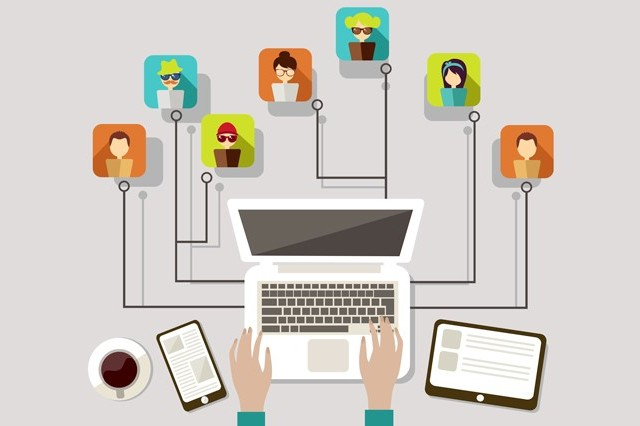
\includegraphics[height=6cm]{immagini/smartworking}
  \end{center}
  \caption{Rappresentazione grafica dello \textit{smart working}.}
  \caption*{\textbf{Fonte:} corriere.it}
\end{figure}

Nonostante la situazione non favorevole, ho avuto comunque modo di interfacciarmi con i dipendenti dell'azienda; sono quindi riuscito anche a raccogliere le informazioni riguardanti l'azienda che, unite a delle ricerche online, ho riportato in questo capitolo.

\section{L'azienda}

Sync Lab nasce come \textit{software house} a Napoli nel 2002; negli anni, l'azienda si espande a gran velocità, aprendo sedi a Roma, Milano, Padova e Verona. Al giorno d'oggi, l'azienda conta 5 sedi, per un totale di oltre 250 dipendenti e più di 150 clienti diretti e finali. \\
Dall'apertura ad oggi, Sync Lab si è tramutata in un \textit{system integrator} grazie alla maturazione delle competenze tecniche e metodologiche in ambito software. Un tratto distintivo dell'azienda è la grande attenzione posta alla gestione delle \textbf{risorse umane}: testimonianza di ciò è il basso \textit{turn-over}, segno che i collaboratori condividono un progetto comune e concreto. \\
Altro segno d'eccellenza sono le certificazioni di qualità che l'azienda ha conseguito; finora, infatti, l'azienda ha ottenuto le certificazioni per gli standard \textit{ISO 9001}, \textit{ISO 14001}, \textit{ISO 27001} e \textit{ISO 45001}. \\

\begin{figure}[htbp]
  \begin{center}
    
\includegraphics[height=1.3cm]{immagini/synclab-logo}
  \end{center}
  \caption{Logo di Sync Lab s.r.l..}
  \caption*{\textbf{Fonte:} synclab.it}
\end{figure}

\subsection*{Prodotti e servizi offerti}

Una certa attenzione è posta dall'azienda alla diversificazione dei prodotti e dei servizi offerti; essi sono infatti inquadrabili in diverse aree tematiche, quali salute, privacy, sicurezza, telecomunicazioni, finanza, territorio e ambiente. \\
Alcuni dei prodotti che l'azienda offre al momento sono i seguenti:

\begin{itemize}
  \item \textbf{DPS 4.0}: software per la gestione degli adempimenti alla \textit{Privacy GDPR - General Data Protection Regulation}, utilizzato da svariate aziende per attuare correttamente quanto previsto da tale regolamento europeo; tale prodotto permette di censire, tracciare e controllare chi può trattare dati personali in azienda;

  \item \textbf{StreamLog}: sistema finalizzato al soddisfacimento dei requisiti fissati dal \textit{Garante per la Protezione dei dati personali}, utilizzato dagli amministratori di sistema per controllare gli accessi agli utenti al fine di soddisfare i requisiti di \textit{privacy} richiesti dal garante;

  \item \textbf{SynClinic}: sistema informativo per la gestione integrata dei processi, clinici e amministrativi, di ospedali, cliniche e case di cura. Questo applicativo fornisce svariate funzionalità, che intersecano i bisogni del personale amministrativo e quelli del personale clinico delle strutture sanitarie, permettendo di gestire e monitorare tutte le fasi del percorso di cura del paziente. È utilizzabile sia in \textit{cloud} che \textit{on premises};

  \begin{minipage}{\linewidth}
    \centering
      
\includegraphics[height=6cm]{immagini/synclinic}
    \captionof{figure}{Moduli di SynClinic.}
    \caption*{\textbf{Fonte:} synclinic.it}
  \end{minipage}

  \item \textbf{StreamCrusher}: tecnologia che aiuta le aziende a effettuare corrette decisioni di \textit{business}, a identificare tempestivamente eventuali criticità e a riorganizzare i processi in base a nuove esigenze. Questo software è in grado di raccogliere, indicizzare e interpretare i dati, siano essi \textit{log} di applicazione o di sistema, \textit{alert}, dati di configurazione o modifiche ai sistemi, al fine di estrapolarne informazioni utili all'\textit{IT management};

  \item \textbf{Wave}: software che si propone come integrazione tra il mondo della videosorveglianza e quello dei \textit{Sistemi Informativi Territoriali}, permettendo di avere una visione geo-referenziata della distribuzione delle telecamere installate sul territorio e consentendo così all'utilizzatore di avere un impatto visivo immediato sull'area di copertura di una data installazione reale, o di avere un'anteprima di tale area in fase di progettazione;

  \item \textbf{Seastream}: piattaforma pensata per migliorare l'efficienza, la sicurezza e il processo di innovazione del settore marittimo; per fare ciò l'azienda fornisce, attraverso questa piattaforma, un \textit{Fleet Operation Center (FOC)}, ovvero un sistema di monitoraggio avanzato delle flotte armatoriali operative in tutto il mondo, e un \textit{Harbor Operation Platform (HOC)}, ovvero una piattaforma di servizi per gli operatori portuali.

  \begin{minipage}{\linewidth}
    \centering
      
\includegraphics[height=4cm]{immagini/seastream}
    \captionof{figure}{Funzionalità del progetto Seastream.}
    \caption*{\textbf{Fonte:} synclab.it}
  \end{minipage}

\end{itemize}

\subsection*{Clienti principali}
Sync Lab collabora con numerose aziende italiane e multinazionali, sia pubbliche che private. Tra le aziende \textbf{private} più importanti possiamo trovare \textit{Sky}, \textit{Eni}, \textit{Enel}, \textit{Vodafone}, \textit{Accenture}, \textit{Fastweb}, \textit{Tim}, \textit{UniCredit} e \textit{H\&M}. \\
Tra le collaborazioni con \textbf{enti statali} e parastatali, invece, troviamo quelle con \textit{Trenitalia}, \textit{RAI}, \textit{Poste Italiane}, la \textit{Regione Lazio} e il \textit{Ministero dell'Economia e delle Finanze}.

%**************************************************************
\section{Processi aziendali}

\subsection{Processi}

L'azienda persegue i propri obiettivi attuando i processi qui elencati.

\subsubsection*{Consulenza}

L'azienda fornisce servizi di consulenza informatica a svariate imprese, sia pubbliche che private; questi servizi hanno lo scopo di far evolvere, sia in termini di sviluppo che di competitività, i clienti dell azienda. Per fare ciò, Sync Lab collabora con altre aziende di consulenza e con specialisti del settore.

\subsubsection*{Fornitura}

Il processo di fornitura viene istanziato ogniqualvolta un cliente assume Sync Lab per lo sviluppo e la realizzazione di un prodotto. Contemporaneamente alla realizzazione, l'azienda svolge delle attività che possano migliorare questo processo. In particolare:
\begin{itemize}
  \item \textbf{Qualità del software}: il software viene controllato e ottimizzato, anche attraverso l'utilizzo delle \textit{best practice}, al fine di aderire alle regole aziendali;
  \item \textbf{Verifica delle procedure}: le procedure vengono verificate, al fine di poter agire in maniera correttiva nel caso in cui si dovessero manifestare dei problemi;
  \item \textbf{Analisi e miglioramento degli standard}: gli standard aziendali vengono analizzati e, possibilmente, migliorati; conseguenza di ciò è un costante miglioramento anche dal punto di vista di qualità del software.
\end{itemize}

\subsubsection*{Sviluppo}

Per quanto riguarda il processo di sviluppo, Sync Lab fa uso della metodologia \textit{Agile}, descritta più dettagliatamente in seguito. Questa permette di coinvolgere il cliente durante tutto il processo, tenendolo aggiornato sull'evoluzione dello sviluppo del prodotto e ricevendo di ritorno le sue opinioni, al fine di poter agire sia correttivamente che migliorativamente.

\subsubsection*{Manutenzione}

Una volta consegnato il prodotto, l'azienda assicura le attività di manutenzione per tutto il ciclo di vita del software. La manutenzione offerta dall'azienda è di tre tipi:
\begin{itemize}
  \item \textbf{Correttiva}, corrispondente alla correzione di eventuali difetti;
  \item \textbf{Adattiva}, ossia il riadattamento del software a nuovi requisiti quali l'ambiente di produzione o l'architettura;
  \item \textbf{Evolutiva}, ossia l'aggiunta o l'aggiornamento in senso migliorativo di porzioni di software.
\end{itemize}

\subsection{Metodologia Agile}

Per il processo di sviluppo, l'azienda fa uso di una metodologia \textit{Agile} che molto si avvicina al modello \textit{Scrum}. Punto cardine del metodo di sviluppo di Sync Lab, infatti, è la continua interazione con gli \textit{stakeholder}, ossia i clienti: questi vengono coinvolti durante tutto il processo, venendo aggiornati sull'evoluzione del prodotto; questo permette all'azienda di ricevere \textit{feedback} che possono aiutare a migliorare il prodotto e ad adattarlo al meglio alle esigenze. \\
Come ho potuto constatare di persona durante il mio periodo di tirocinio, il modello adottato dall'azienda prevede uno sviluppo che procede per \textit{sprint}, ossia un'unità di base di durata fissa compresa tra una e quattro settimane a seconda degli obiettivi posti. A ogni \textit{sprint} corrisponde una funzionalità; questa viene verificata insieme al cliente, per tastarne la soddisfazione o ricevere consigli che possano migliorare tale nuova funzionalità. \\

\begin{minipage}{\linewidth}
  \centering
    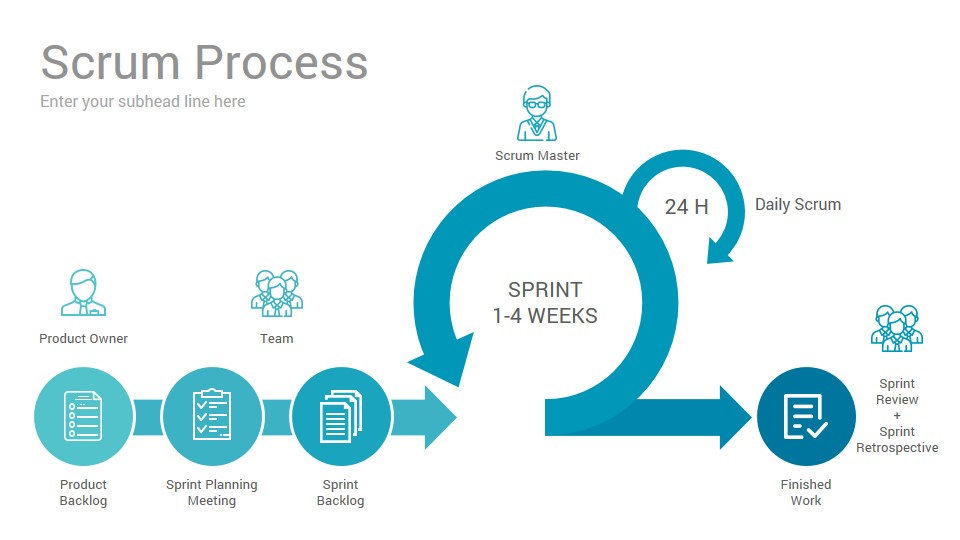
\includegraphics[height=6cm]{immagini/scrum}
  \captionof{figure}{Metodologia Scrum.}
  \caption*{\textbf{Fonte:} antevenio.com}
\end{minipage}

Lo sviluppo di un prodotto in Sync Lab passa attraverso cinque attività, inquadrabili tutte in quanto previsto dalla metodologia \textit{Scrum}. \\
La prima attività che viene svolta è la redazione di una lista di cose da fare per portare a termine il progetto; nel caso del mio progetto di \textit{stage}, ad esempio, ho definito insieme al tutor aziendale le \textit{feature} che avrei dovuto implementare, e abbiamo visionato assieme i \textit{bug} presenti nel codice che avrei dovuto utilizzare come \textit{baseline}, al fine di sapere cosa avrei dovuto correggere di quanto già fatto. Nella metodologia \textit{Scrum}, questa lista assume il nome di \textbf{Product Backlog}. \\
Dopo aver redatto questa lista, solitamente viene realizzata una pianificazione degli \textit{sprint} che è necessario effettuare per portare a termine il progetto. In ambito \textit{Scrum} questa pianificazione viene chiamata \textbf{Sprint Planning}, e nel caso del mio tirocinio è corrisposta alla divisione in incrementi che avrei dovuto effettuare per completare il piano di lavoro. Successivamente a questo, vengono individuati dei sottoinsiemi di obiettivi per ogni \textit{sprint} definito durante l'attività chiamata \textbf{Sprint Backlog}. Un esempio pratico di questa attività è la definizione degli incrementi che ho effettuato prima di cominciare lo \textit{stage}. \\
Una volta definiti tutti gli obiettivi e aver correttamente diviso le tempistiche in \textbf{Sprint}, questi vengono ad uno ad uno eseguiti; nell'ambito del mio stage, questo è corrisposto allo sviluppo di quanto previsto dal piano di progetto. All'esecuzione di ogni incremento, inoltre, di questo è stata verificata l'aderenza agli obiettivi posti, che nella metodologia \textit{Scrum} vegnono chiamati \textbf{Sprint Goal}.

Durante il mio \textit{stage} ho inoltre potuto sperimentare anche due degli eventi facenti parte della metodologia \textit{Scrum}, ossia il \textit{Daily Scrum} e lo \textit{Sprint Review}:
\begin{itemize}
  \item Il \textbf{Daily Scrum}, come definito dai creatori di questa metodologia, è un evento a cadenza giornaliera in cui i membri del gruppo di lavoro discutono dell'andamento dello \textit{sprint}. Questo evento viene svolto dai diversi \textit{team} di lavoro dell'azienda giornalmente; nel caso specifico del mio tirocinio, essendosi questo svolto in gran parte in \textit{remote working}, questo evento non ha potuto avere cadenza giornaliera. Nonstante questo, ho effettuato svariati allineamenti con il tutor aziendale, e questo si può almeno in parte configurare con quanto previsto dalla metodologia;
  \item Lo \textbf{Sprint Review}, ossia la verifica di quanto effettuato durante uno \textit{sprint} alla fine di questo, viene effettuato da tutti i gruppi di lavoro al raggiungimento degli obiettivi fissati dallo \textit{sprint}. Nel caso specifico del mio tirocinio, questo evento ha avuto luogo quasi settimanalmente, con la verifica di quanto fatto durante l'incremento definito.
\end{itemize}

%**************************************************************

\section{Tecnologie utilizzate}

Sync Lab fa uso di diversi linguaggi di programmazione, \textit{framework} e strumenti di supporto moderni e funzionali, al fine di soddisfare i clienti; oltre a questo, l'azienda è costantemente aggiornata sulle tecnologie di riferimento e pronta ad espandere le proprie conoscenze con le tecnologie più moderne. \\

\begin{minipage}{\linewidth}
  \centering
    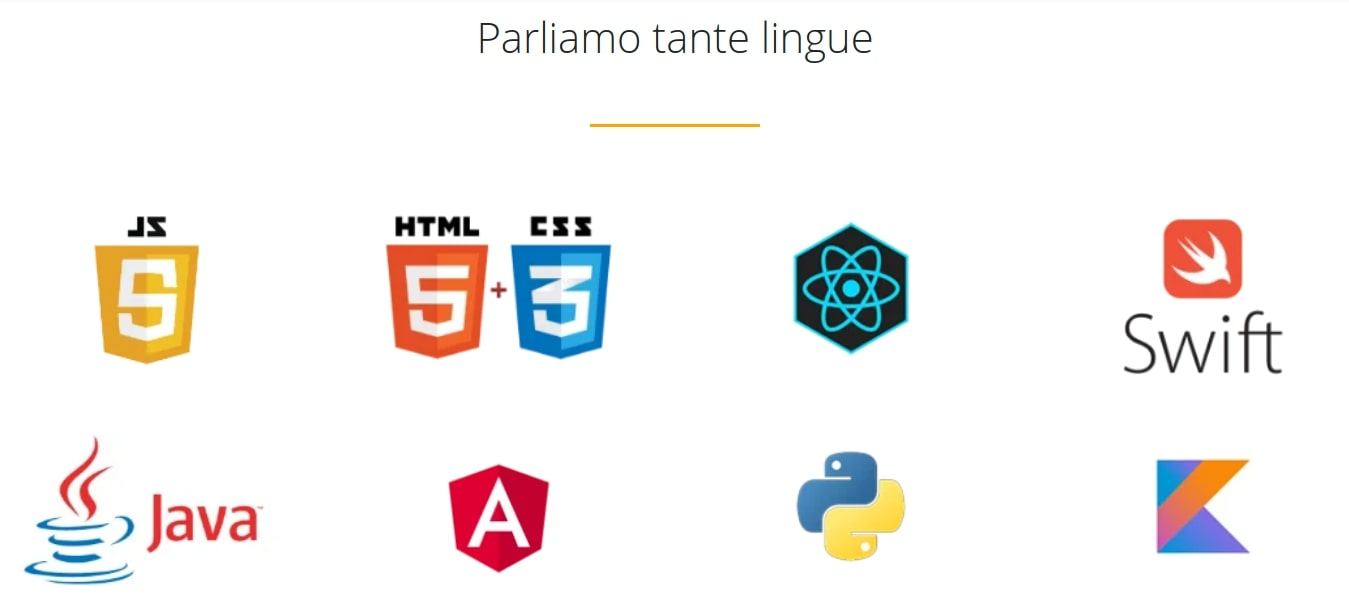
\includegraphics[height=5cm]{immagini/linguaggi}
  \captionof{figure}{Panoramica delle tecnologie utilizzate da Sync Lab.}
  \caption*{\textbf{Fonte:} synclab.it}
\end{minipage} \newpage

Tra i linguaggi di programmazione più utilizzati troviamo i seguenti:
\begin{itemize}
  \item \textbf{Java}: linguaggio di programmazione ad alto livello orientato agli oggetti, largamente utilizzato dalle aziende; in particolare, \textit{Java} viene utilizzato da Sync Lab, in accoppiata al \textit{framework Spring}, per lo sviluppo dei servizi \textit{REST} necessari alle componenti \textit{back-end} di svariati applicativi, tra cui ad esempio \textit{SynClinic} e \textit{StreamCrusher}. Questo linguaggio, abbinato al \textit{framework Spring}, è stato utilizzato anche per lo sviluppo della componente \textit{back-end} dell'applicativo \textit{SyncTrace}, oggetto del mio tirocinio;

  \item \textbf{JavaScript}: linguaggio di programmazione orientato agli oggetti e agli eventi, originariamente pensato per la creazione di effetti dinamici interattivi per i siti web ma sempre più utilizzato come linguaggio \textit{general purpose} per lo sviluppo di applicativi web e non web. Viene utilizzato dall'azienda per realizzare la componente logica delle \textit{Single Page Application};

  \item \textbf{TypeScript}: \textit{super-set} di \textit{JavaScript} sviluppato da \textit{Microsoft}. Questo linguaggio estende la sintassi di \textit{JavaScript} in modo che ogni programma scritto in \textit{JavaScript} possa funzionare anche con \textit{TypeScript}, e come il primo viene utilizzato dall'azienda per realizzare la componente logica delle \textit{Single Page Application}. Si può trovare questo linguaggio, abbinato al \textit{framework Angular}, in svariati prodotti dell'azienda, tra cui \textit{SynClinic} e \textit{DPS4.0}; è inoltre il linguaggio con il quale è stata scritta la componente \textit{front-end} della \textit{web application} di \textit{SyncTrace};

  \item \textbf{HTML5 e CSS3}: linguaggi di \textit{markup} utilizzati, anche dall'azienda, per modellare la componente visiva delle \textit{Single Page Application} e, più in generale, dei siti web. Questi linguaggi di \textit{markup} sono usati dall'azienda principalmente nei progetti che coinvolgono il \textit{framework Angular}, come ad esempio \textit{SynClinic} e \textit{DPS4.0};

  \item \textbf{Kotlin}: linguaggio di programmazione \textit{general purpose} e multi-paradigma, sviluppato da \textit{JetBrains}, utilizzato dall'azienda per sviluppare le applicazioni mobili per i dispositivi \textit{Android}. Un esempio di utilizzo di questo linguaggio è l'applicazione mobile per il \textit{contact tracing} del progetto \textit{SyncTrace};

  \item \textbf{Swift}: linguaggio di programmazione orientato agli oggetti, sviluppato da \textit{Apple} e utilizzato dall'azienda per sviluppare le applicazioni mobili per i dispositivi \textit{iOS}.
\end{itemize}

L'azienda utilizza anche svariati \textit{framework} a supporto della programmazione; alcuni tra i \textit{framework} più utilizzati dall'azienda sono:
\begin{itemize}
  \item \textbf{Spring}: \textit{framework open-source} per lo sviluppo di applicazioni con linguaggio di programmazione \textit{Java}; viene utilizzato, possibilmente combinando il \textit{core} del \textit{framework} con altri progetti quali \textit{Spring Boot} e \textit{Spring Data}, per sviluppare applicativi lato \textit{server}. Esempio di utilizzo di questo \textit{framework} da parte di Sync Lab sono svariate applicazioni web la cui componente \textit{back-end} è sviluppata con l'ausilio di queste tecnologie, come ad esempio \textit{SynClinic} e \textit{StreamCrusher};

  \begin{minipage}{\linewidth}
    \centering
      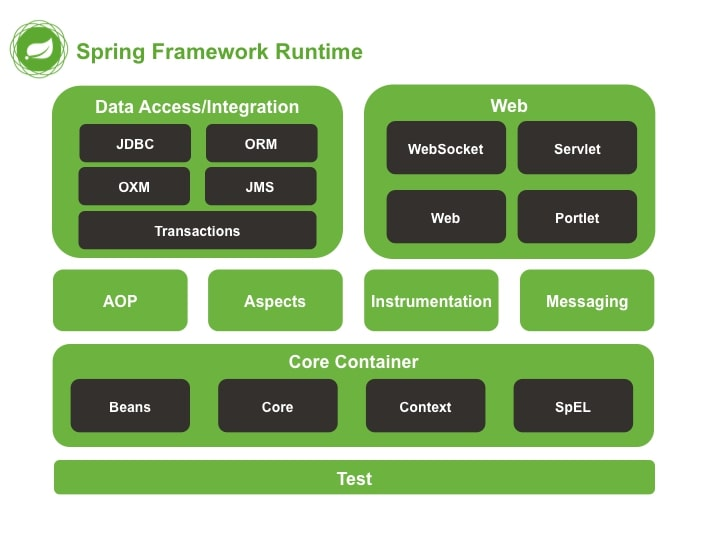
\includegraphics[height=5cm]{immagini/spring}
    \captionof{figure}{Architettura dello \textit{Spring framework}.}
    \caption*{\textbf{Fonte:} javaboss.it}
  \end{minipage}

  \item \textbf{Angular}: \textit{framework open-source} per lo sviluppo di applicazioni web tramite linguaggio di programmazione \textit{TypeScript}. L'utilizzo principale di questa tecnologia risiede nello sviluppo di \textit{Single Page Application} reattive e costruite su un \textit{back-end} composto da servizi \textit{REST}. Esempi di utilizzo di questo \textit{framework} sono \textit{SynClinic} e \textit{DPS4.0}, già citati in precedenza. \\
  Oltre alla possibilità di sviluppare applicativi veloci e funzionali, questo \textit{framework} offre anche un \textit{design pattern} di tipo \textit{Model-View-ViewModel} nativo, fattore che facilita la progettazione e lo sviluppo delle applicazioni;

  \begin{minipage}{\linewidth}
    \centering
      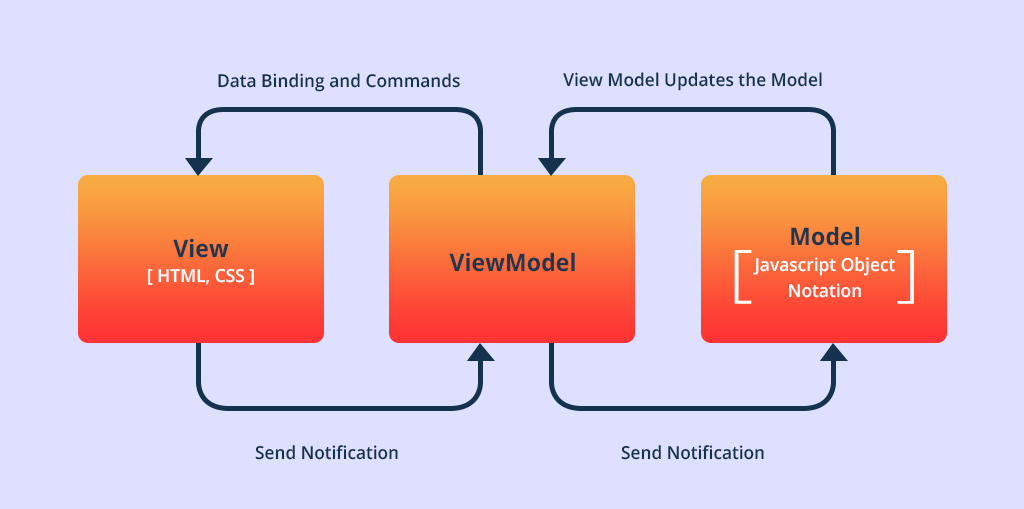
\includegraphics[height=5cm]{immagini/angular}
    \captionof{figure}{Pattern MVVM, adottato anche dal \textit{framework Angular}.}
    \caption*{\textbf{Fonte:} alphalogicinc.com}
  \end{minipage}

  \item \textbf{Electron}: \textit{framework open-source} che consente lo sviluppo dell'interfaccia grafica di applicazioni desktop utilizzando tecnologie tipicamente pensate per il web, quali \textit{HTML}, \textit{CSS}, \textit{JavaScript} e \textit{TypeScript}; per fare ciò, questa tecnologia combina il motore di rendering \textit{Chromium} e il \textit{runtime} \textit{NodeJS}.

  \begin{minipage}{\linewidth}
    \centering
      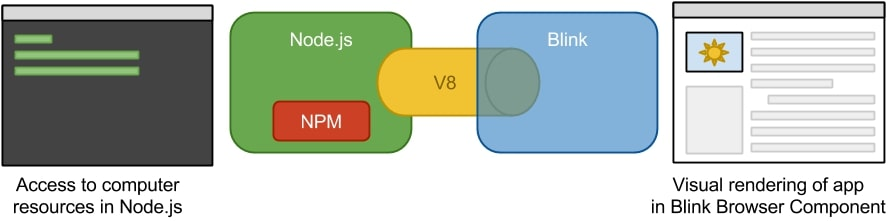
\includegraphics[height=2cm]{immagini/electron}
    \captionof{figure}{Funzionamento del \textit{framework Electron} con \textit{NodeJS}.}
    \caption*{\textbf{Fonte:} freecontent.manning.com}
  \end{minipage}
\end{itemize}

Sync Lab utilizza strumenti tecnologici anche per gestire il lavoro da remoto; in particolare, durante l'emergenza sanitaria ancora in corso, l'azienda fa uso di diverse tecnologie per organizzare il lavoro non in presenza, permettendo a tutti i collaboratori di rimanere correttamente aggiornati sulle attività e i compiti di cui sono responsabili. Alcune di queste tecnologie sono le seguenti:

\begin{itemize}
  \item \textbf{Google Meet}: servizio di \textit{Google} per effettuare videoconferenze online. Questa piattaforma viene usata dall'azienda, e in particolare è stata utilizzata anche durante il mio \textit{stage}, per comunicare con gli altri collaboratori e poter rimanere aggiornati sui progressi effettuati;

  \item \textbf{Discord}: applicazione \textit{VoIP} per la comunicazione vocale e testuale. Uno dei punti di forza di questa piattaforma, sfruttato anche dall'azienda, è la possibilità di poter avere più canali, sia testuali che vocali, all'interno dello stesso \textit{server}; questo permette una comunicazione più ordinata e metodica, riducendo il rischio di incomprensioni;

  \item \textbf{Google Docs}: servizio di \textit{Google} per la condivisione di documenti online. Questa piattaforma è stata utilizzata in particolare durante il mio tirocinio per tenere traccia degli incrementi giornalieri che ho svolto;

  \item \textbf{Trello}: software gestionale in stile \textit{Kanban}, utilizzato per coordinare il proprio \textit{workflow} e visualizzare quello degli altri collaboratori. Questa piattaforma si sposa bene con la metodologia \textit{Agile} che Sync Lab utilizza, in quanto può essere utilizzato come una \textit{Scrum board}.
\end{itemize}

%**************************************************************

\section{Propensione all'innovazione}

Sync Lab presta grande attenzione anche all'innovazione e allo sviluppo, sia in senso tecnologico che industriale. L'azienda, infatti, conta tre dipartimenti ideati per sperimentare e innovare, i quali sono \textbf{Research and Development}, nato con lo scopo di promuovere nuovi prodotti nati da ricerche in svariati settori, \textbf{Lab}, in cui l'azienda sviluppa soluzioni a quanto studiato nel precedente dipartimento, e \textbf{Start-up}, il cui scopo è quello di promuovere le \textit{start-up} di maggiore rilevanza per quanto riguarda l'innovazione; per fare ciò, Sync Lab collabora con svariati enti privati e università, sia italiane che estere.

\begin{minipage}{\linewidth}
  \centering
    
\includegraphics[height=2cm]{immagini/universita}
  \captionof{figure}{Alcune università con le quali l'azienda collabora.}
  \caption*{\textbf{Fonte:} synclab.it}
\end{minipage}

Alcuni dei progetti di ricerca fondati e mantenuti da Sync Lab sono i seguenti:
\begin{itemize}
  \item \textbf{BIG-ASC}: acronimo di \textit{BIG Data and Advanced Analytics for Secure Mobile Commerce}, è un progetto che punta a creare una piattaforma \textit{Big Data} che sappia rispondere a requisiti stringenti delle piattaforme di \textit{Mobile Commerce}, come la scalabilità, l'autonomia e le performace, attraverso l'analisi continua e in tempo reale dei dati d'utilizzo. Per fare questo, Sync Lab collabora con l'azienda \textit{CeRICT} e l'\textit{Università degli studi Parthenope} di Napoli;
  \item \textbf{eHealthNet}: ecosistema software per la Sanità Elettronica, che si propone di intervenire su quattro aree tematiche riguardanti la sanità, ossia interoperabilità, pervasività, sostenibilità e preventivabilità. Per lo sviluppo di questo progetto è stato avviato un laboratorio che vede come collaboratori svariate aziende private, l'\textit{Istituto Italiano di Tecnologia}, l'\textit{Istituto Nazionale Tumori}, l'\textit{Università degli studi Federico II} di Napoli e l'\textit{Università degli studi di Salerno};
  \item \textbf{BDA4PHR}: piattaforma \textit{open-source}, scalabile, estendibile e manutenibile che offre servizi di \textit{storing} e \textit{Big Data Analytics} dedicati ad informazioni di tipo medico-sanitario. Scopo di questo progetto è la creazione di un \textit{repository} sicuro, distribuito e affidabile per la gestione, la condivisone e l'analisi di dati eterogenei. Tra i finanziatori di questo progetto ci sono l'\textit{Unione Europea} e il \textit{Ministero dello Sviluppo Economico} italiano.
\end{itemize}

\begin{minipage}{\linewidth}
  \centering
    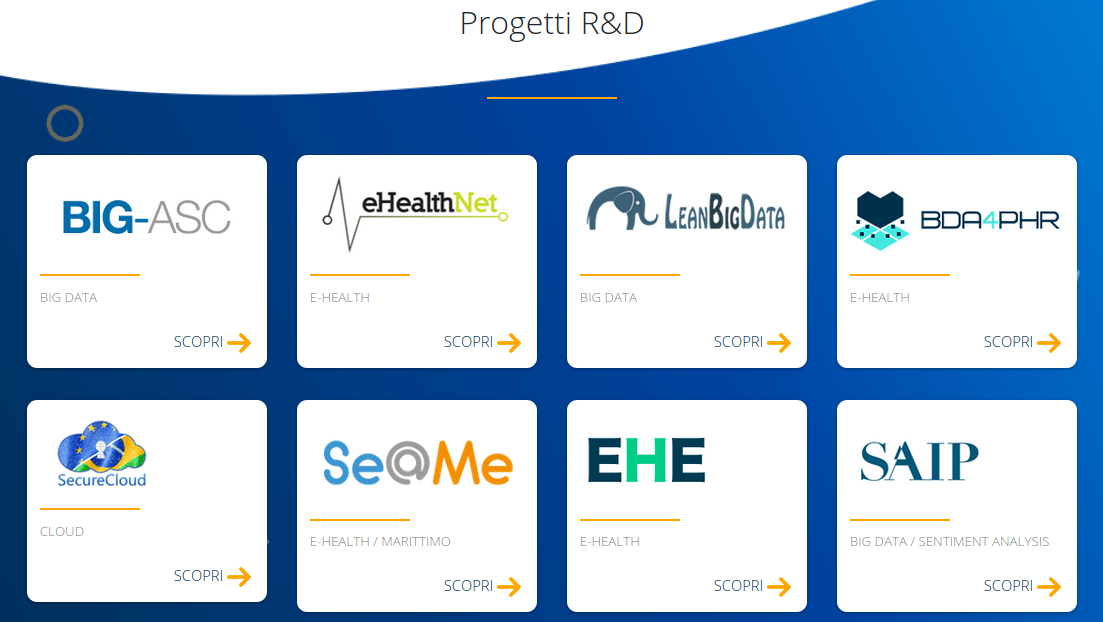
\includegraphics[height=5.5cm]{immagini/progetti}
  \captionof{figure}{I progetti di ricerca e sviluppo a cui Sync Lab collabora.}
  \caption*{\textbf{Fonte:} synclab.it}
\end{minipage}

Sempre nell'ambito dell'innovazione, posso dire che l'azienda ha un atteggiamento molto propositivo e aperto alle nuove tecnologie: non è raro, infatti, che i collaboratori propongano l'utilizzo di nuovi linguaggi, \textit{framework} e strumenti per completare i servizi e i prodotti offerti dall'azienda. \\
Ho potuto respirare questo clima di apertura anche nell'ambito del mio tirocinio: avendo avuto accesso alla piattaforma \textit{Discord} aziendale, ho potuto notare che il \textit{server} è diviso in più sottocanali, ognuno dedicato a un ambito di sviluppo, in cui i dipendenti inoltrano articoli e documentazione riguardanti nuove tecnologie, aprendo così a un dibattito costruttivo.

% !TEX encoding = UTF-8
% !TEX TS-program = pdflatex
% !TEX root = ../tesi.tex

%**************************************************************
\chapter{Il progetto nel contesto aziendale}
\label{cap:progetto-contesto-aziendale}
%**************************************************************

\section{Il rapporto tra stage e azienda}

Lo \textit{stage} è un momento fondamentale nella carriera di uno studente universitario; esso infatti rappresenta un passaggio dal mondo accademico al mondo del lavoro, permettendo di passare gradualmente da un'ottica di studio prettamente teorico, per quanto corredato da esercizi pratici, a un'ottica di lavoro con tecnologie, strumenti e metodologie utilizzate quotidianamente dalle aziende. \\

\begin{minipage}{\linewidth}
  \centering
    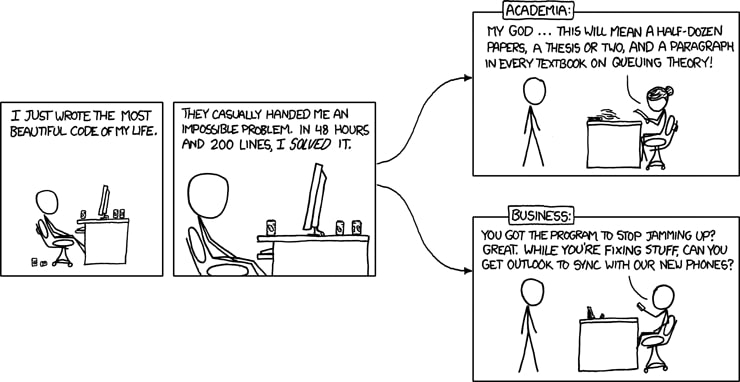
\includegraphics[height=3.8cm]{immagini/academiavsbusiness}
  \captionof{figure}{\textit{Academia vs business - xkcd}.}
  \caption*{\textbf{Fonte:} xkcd.com}
\end{minipage} \\

Sync Lab, avendo sedi in città universitarie ed essendo sempre tesa verso l'innovazione, prende con gran serietà l'opportunità di ospitare tirocini al suo interno. Questo si può vedere dalla grande \textbf{esperienza} che questa azienda ha in fatto di \textit{stage}: essi sono infatti organizzati in modo da conformarsi al meglio alle esigenze dello studente, in quanto molto flessibili in termini di durata complessiva. In Sync Lab, inoltre, lo studente non solo è seguito da un tutor esterno, che si occupa di guidare il tirocinante sia organizzativamente che pragmaticamente durante lo sviluppo, ma può trovare aiuto e consiglio anche negli altri collaboratori dell'ufficio. \\
Per quanto riguarda le motivazioni che ha Sync Lab ad ospitare \textit{stage} universitari, ho individuato le seguenti:
\begin{itemize}
  \item Prima tra tutte è la tendenza all'\textbf{innovazione}: uno studente universitario, infatti, per quanto inesperto della vita lavorativa è mediamente più aggiornato sulle nuove tecnologie, e questo porta l'azienda ad aprirsi a nuove tematiche;
  \item C'è poi un'ottica di \textbf{assunzione futura}: le università sono infatti per Sync Lab il principale bacino di nuovi lavoratori. È molto frequente, infatti, che dopo un tirocinio ben riuscito l'azienda offra un contratto di lavoro allo studente, se questi è disponibile al lavoro;
  \item Infine, un aspetto da prendere in considerazione è quello \textbf{economico}: l'azienda, infatti, non è obbligata a pagare un rimborso spese al tirocinante, e la maggior parte delle spese assicurative sono a carico dell'università; la presenza di uno o più tirocinanti, infine, non rappresenta un costo rilevante in termini di risorse.
\end{itemize}

%**************************************************************

\section{L'azienda in relazione al contesto attuale}

Il 31 dicembre 2019, le autorità cinesi riferiscono all'\textit{Organizzazione Mondiale della Sanità} di 41 casi di polmonite anomala che si sono verificati a Wuhan, capitale della provincia di Hubei, in Cina; pochi giorni dopo, gli scienziati cinesi identificano il nuovo virus con il nome di \textit{2019-nCov}. Inizialmente, tutto il mondo sottovaluta questa situazione, pensando che fosse un problema riguardante solo la Cina e pochi altri paesi del sud-est asiatico; il 31 gennaio 2020, però, vengono confermati i primi due casi di contagio in Italia.\footcite{sole24ore:cronistoria-covid} Da quel momento, la sensazione che potesse diventare un problema globale comincia a farsi strada nei pensieri di molte persone. \\
I giorni a seguire vedono una rapida successione di eventi: a inizio febbraio il virus viene rinominato dall'\textit{OMS} in \textit{SARS-CoV-2}, a fine febbraio scattano le cosiddette \textbf{zone rosse} in Italia, zone da cui diventa impossibile uscire e in cui è impossibile entrare, il 7 marzo la Lombardia diventa totalmente zona rossa e, due giorni dopo, scatta il \textit{lockdown} in tutta Italia\footcite{sole24ore:cronistoria-covid}. Da questo momento, la maggior parte dei luoghi di lavoro viene chiusa, e questo \textit{shutdown} dura fino all'introduzione della \textit{fase 2}, il 4 maggio, giorno in cui alcune attività vengono riavviate, e ancora parzialmente fino al 15 giugno, giorno in cui scatta la \textit{fase 3} che durerà fino al 13 ottobre. \\

\begin{minipage}{\linewidth}
  \centering
    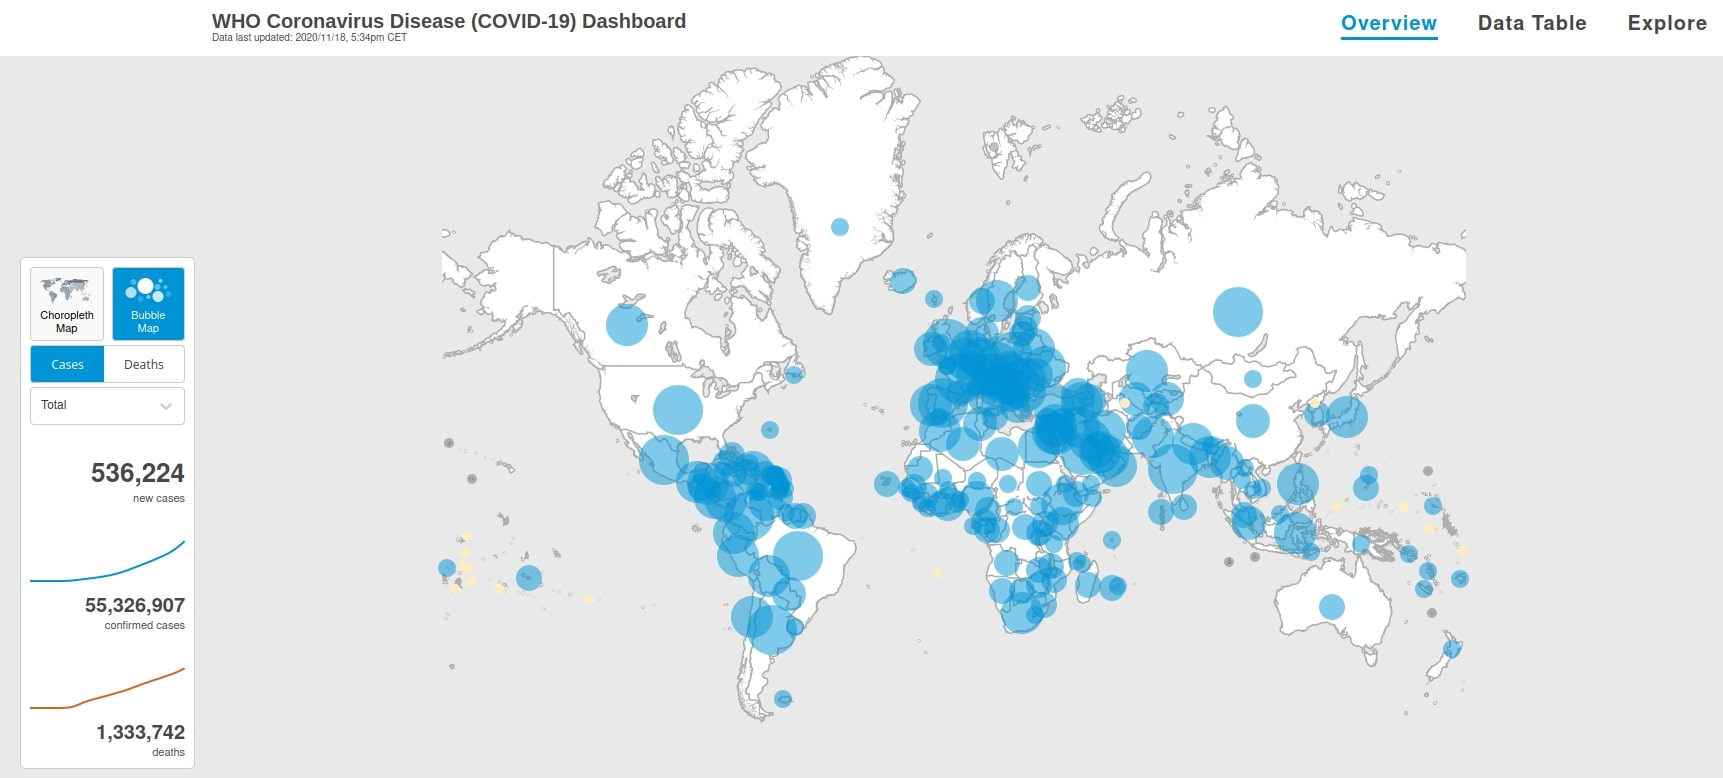
\includegraphics[height=4.5cm]{immagini/covid}
  \captionof{figure}{\textit{Dashoard} di COVID-19 nel mondo.}
  \caption*{\textbf{Fonte:} covid19.who.int}
\end{minipage} \\

Durante questo periodo di emergenza sanitaria, molte aziende cominciano ad adottare le tecniche del \textit{remote working} e dello \textit{smart working}; tra queste aziende c'è anche Sync Lab, che si attrezza per permettere ai suoi dipendenti e ai tirocinanti di lavorare da casa, interrompendo inizialmente e riducendo di molto successivamente la presenza fisica negli uffici. \\
Questo contesto di attualità è di grande importanza anche per quanto riguarda il mio \textit{stage} in particolare: temporalmente parlando, infatti, il mio tirocinio è coinciso con la cosiddetta fase 3. Sebbene fosse possibile effettuare incontri fisici, l'azienda ha infatti deciso di ridurre tali incontri per una questione di sicurezza; da questo ne deriva che ho svolto gran parte del mio tirocinio da casa, senza poter accedere direttamente alle strutture e alle infrastrutture se non una volta alla settimana. \\
Oltre a questo, il periodo è altresì di vitale importanza per descrivere lo \textbf{scopo} del mio tirocinio: come descrivo più approfonditamente nella sezione seguente, infatti, il progetto di \textit{stage} si configura all'interno del progetto \textit{SyncTrace}, un insieme di applicativi concernenti il tema del \textit{contact tracing}.

%**************************************************************

\section{Lo scopo dello stage}

In risposta alla situazione sanitaria, molte aziende del settore \textit{ICT} si sono attivate per sviluppare applicazioni e sistemi di \textit{contact tracing}. Il \textit{contact tracing} consiste nell'identificazione delle persone che potrebbero essere venute a contatto con una persona infetta, e nella successiva raccolta di ulteriori informazioni, quali vicinanza e tempo di esposizione, su tali contatti; il fine di questa pratica è aiutare il sistema sanitario a individuare i possibili contagi, arrivando a costruire un albero dei contatti per poter agire tempestivamente sul problema. \\

\begin{minipage}{\linewidth}
  \centering
    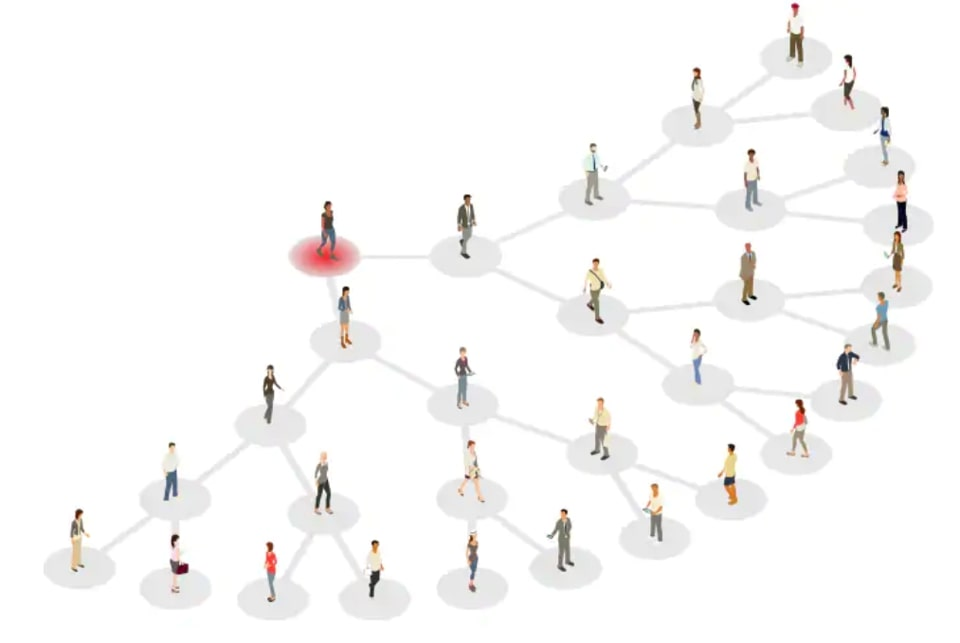
\includegraphics[height=5cm]{immagini/contacttracing}
  \captionof{figure}{Rappresentazione schematica del \textit{contact tracing}.}
  \caption*{\textbf{Fonte:} mashable.com}
\end{minipage} \\

Tra le aziende che si sono mobilitate per questa causa c'è anche Sync Lab, che ha avviato un suo progetto in tale ambito chiamato \textit{SyncTrace}. Questo sistema ha come scopo lo sviluppo di due prodotti differenti ma in relazione tra loro: un'applicazione di \textit{contact tracing} puro e un applicativo di gestione e organizzazione per i medici e per gli esercenti di attività commerciali. \\
Il \textbf{primo} applicativo, pensato per l'utilizzo da parte di tutta la popolazione, ha come unico scopo il tracciamento dei contatti delle persone infette; esso è in forma di applicazione per dispositivi mobili, quali \textit{smartphone} e \textit{tablet}, ed è pensato in modo da tracciare i contatti e i livelli di rischio di positività basandosi su parametri oggettivi come la vicinanza e il tempo di esposizione. \\

\begin{minipage}{\linewidth}
  \centering
    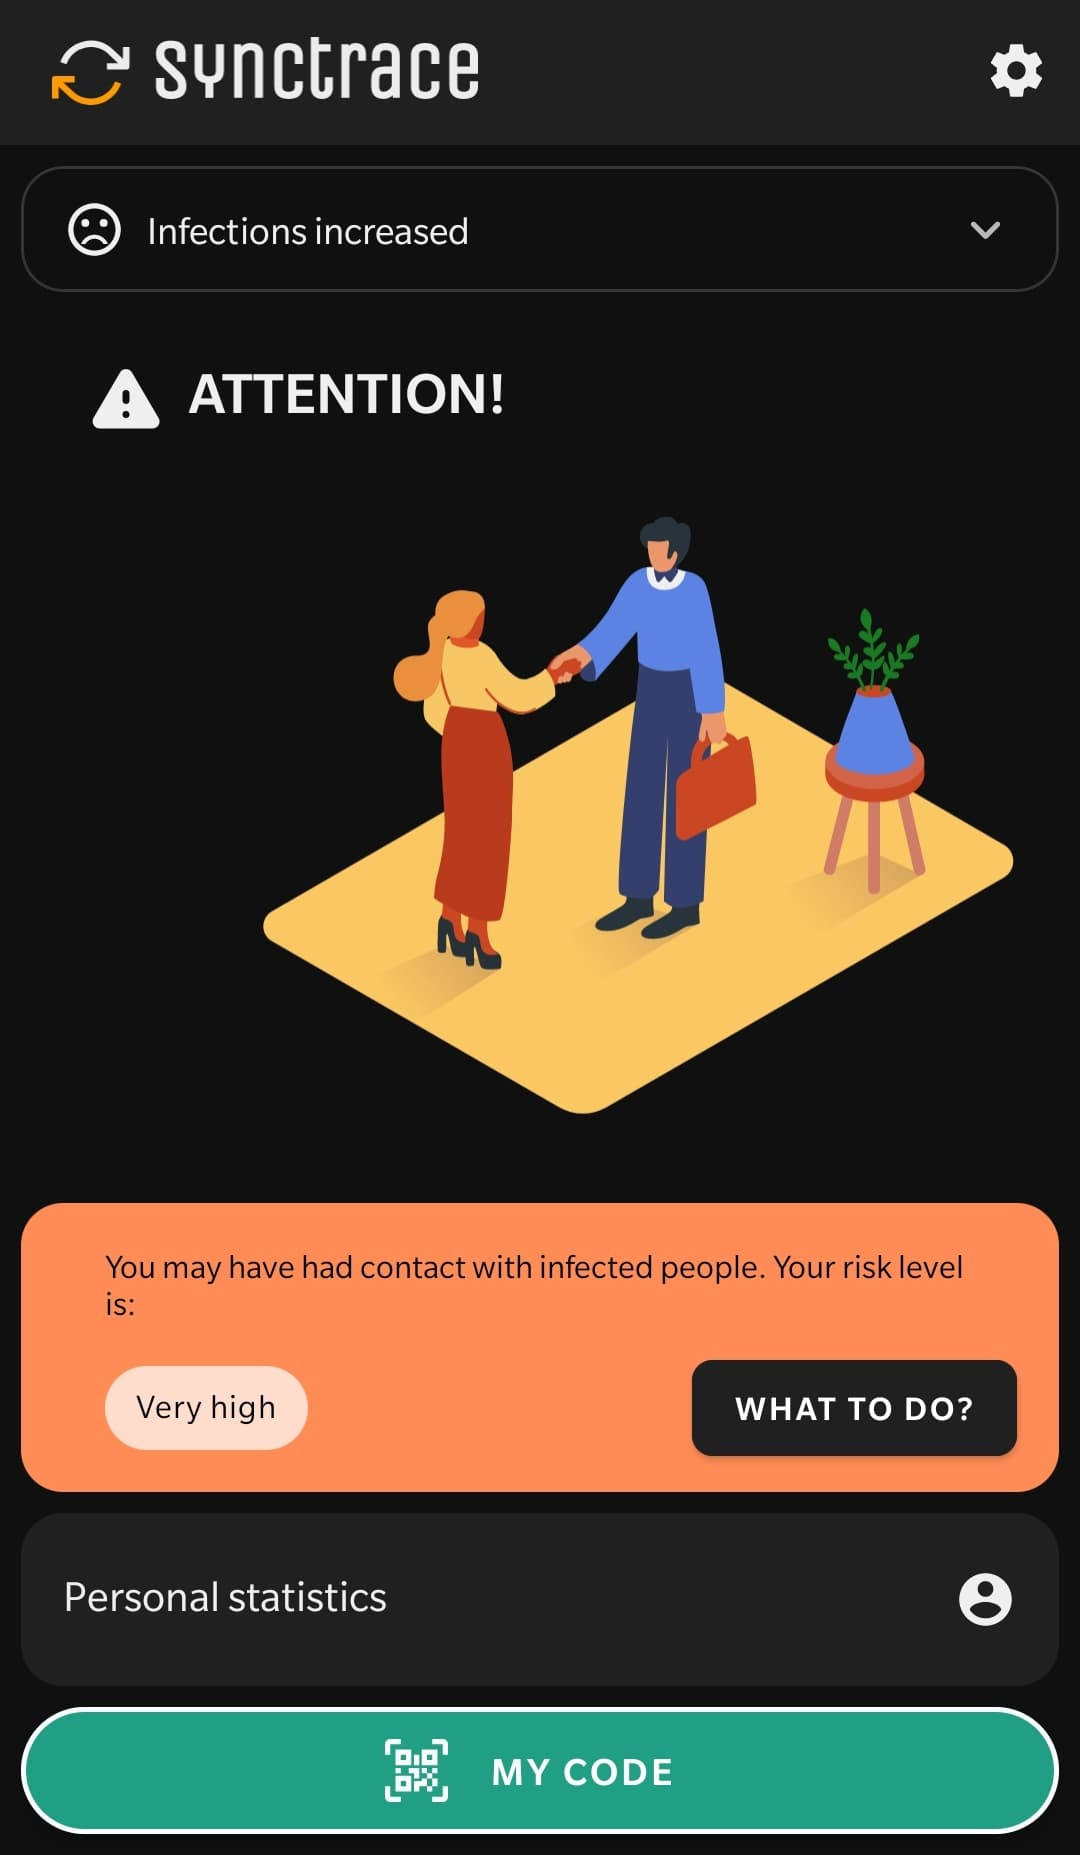
\includegraphics[height=7cm]{immagini/synctraceandroid}
  \captionof{figure}{Schermata iniziale dell'applicazione \textit{SyncTrace}.}
\end{minipage} \\

Il \textbf{secondo} applicativo, consistente in una \textit{web application}, è pensato per fornire un'interfaccia di gestione del sistema ai medici e come applicazione di controllo per gli esercenti. Esso ha quindi un doppio utilizzo:
\begin{itemize}
  \item I \textbf{medici}, una volta identificati come tali, possono usarlo per registrare nuovi contatti infetti, eliminare eventuali pazienti non infetti e verificarne la presenza e/o il livello di rischio di contagio nel sistema condiviso;
  \item Gli \textbf{esercenti}, una volta registrati come tali, possono controllare l'eventuale positività o il livello di rischio di contagio dei clienti che entrano nelle proprie attività.
\end{itemize}

\begin{minipage}{\linewidth}
  \centering
    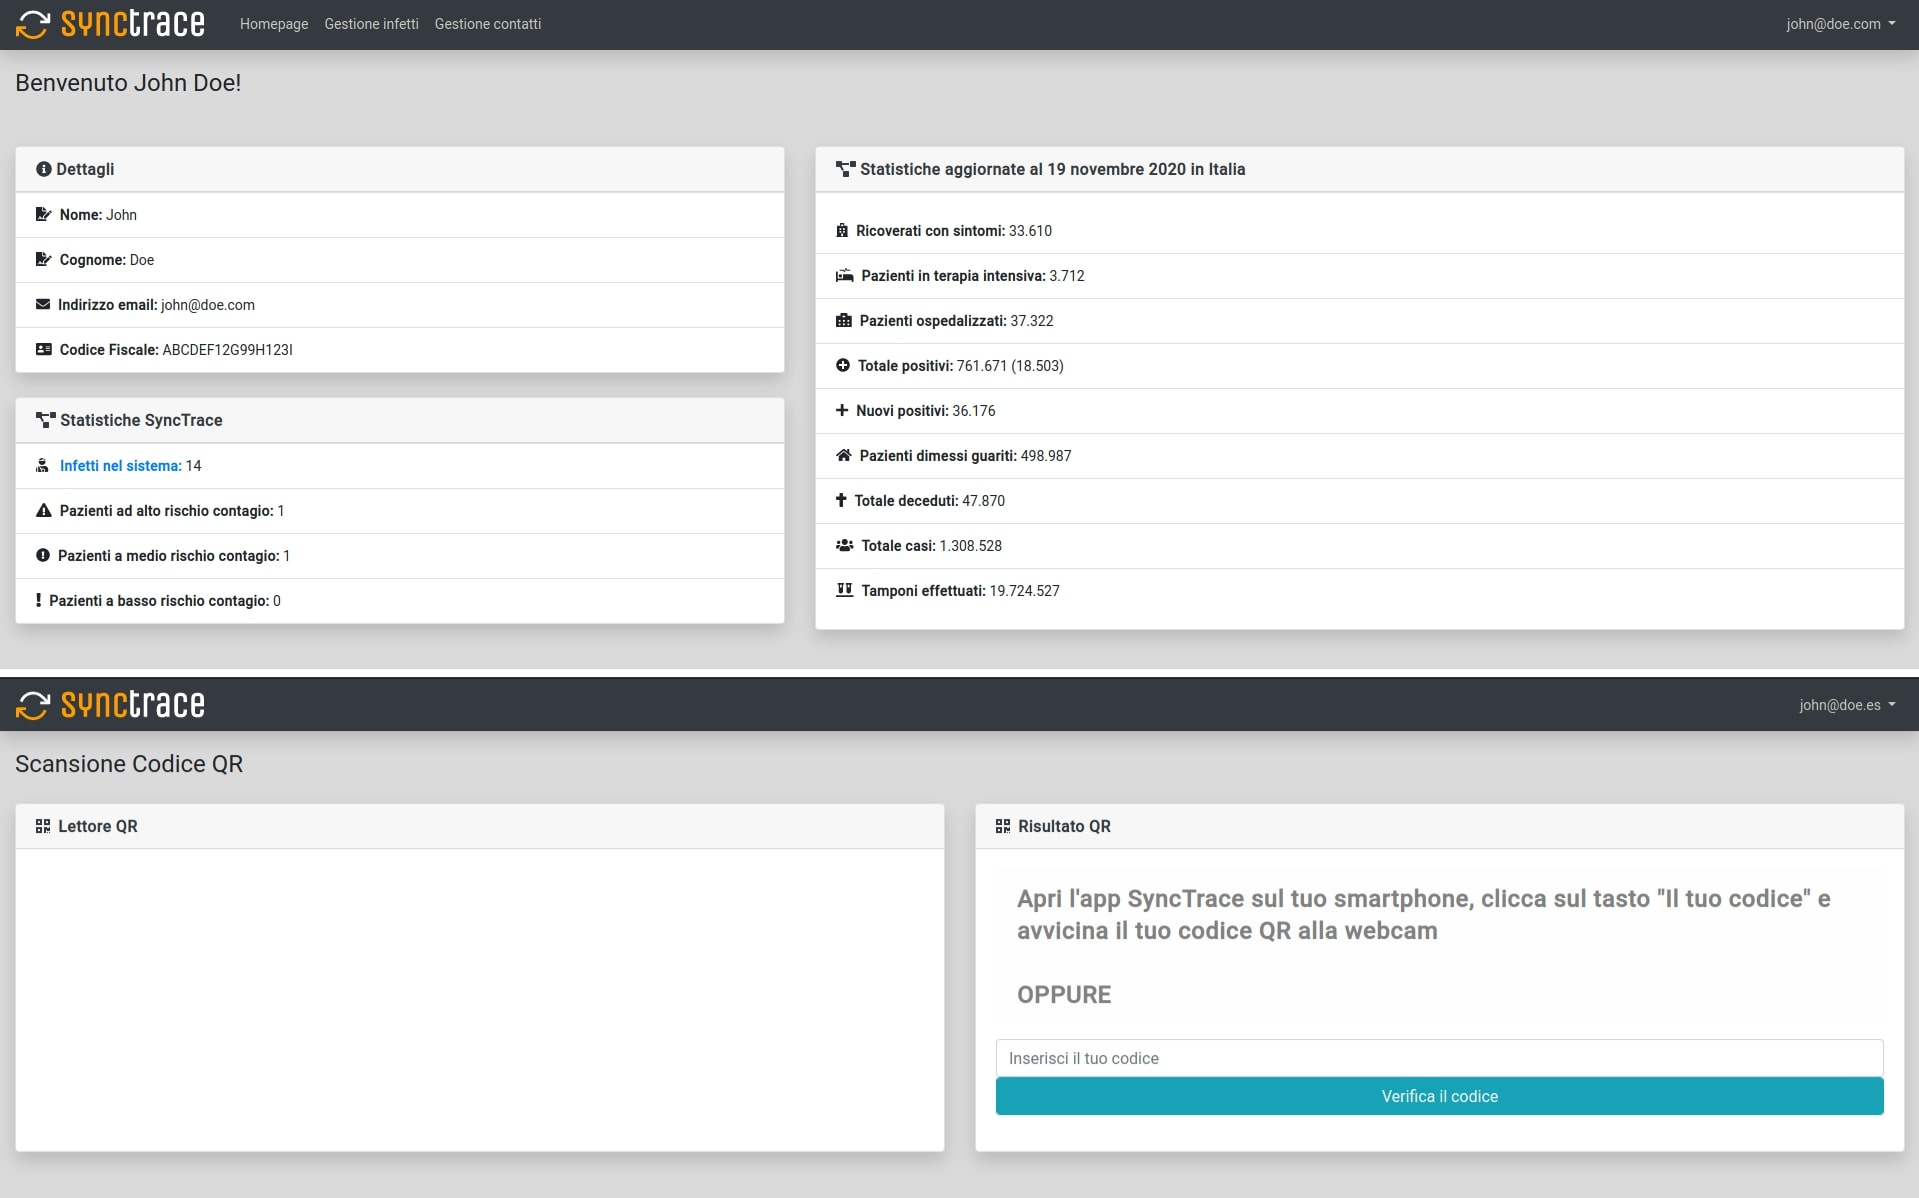
\includegraphics[height=5cm]{immagini/webapp}
  \captionof{figure}{Schermata iniziale della \textit{webapp} per, rispettivamente, medici ed esercenti.}
\end{minipage} \\

Il mio progetto di \textit{stage} si inserisce nel contesto di quest'ultimo applicativo descritto. Lo scopo principale del mio tirocinio è, infatti, effettuare il \textit{porting} dell'applicativo utilizzando il \textit{framework Ionic}, per poter riutilizzare parte della logica già sviluppata secondo il principio del \textit{write once, run anywhere}.

%**************************************************************

\section{Vincoli e obiettivi dello stage}

Prima di cominciare il tirocinio ho definito, insieme al tutor aziendale Andrea Giunta, gli obiettivi e i vincoli che il mio lavoro avrebbe dovuto rispettare. Questo ha portato alla stesura di un \textbf{piano di lavoro}, riportante lo scopo dello stage, i prodotti attesi, la pianificazione settimanale del lavoro e gli obiettivi del progetto; durante il progetto, però, questo piano di lavoro ha subito due modifiche per meglio adattarsi a esigenze personali e per occupare al meglio il tempo in termini di produttività.

\subsection{Vincoli temporali}

Inizialmente, lo \textit{stage} aveva una durata prevista di 8 settimane, di cui 7 da 40 ore l'una e l'ultima da 20 ore, per un totale di 300 ore. A causa di malattia personale, però, non ho potuto effettuare la penultima settimana come previsto, e ho dovuto quindi effettuare una nona settimana per concludere le 300 ore previste e, con esse, quanto previsto dal piano di lavoro. Il totale di ore è stato quindi \textbf{308}. \\
Come già detto, la maggior parte del progetto si è svolto in \textit{smart working}: ho quindi lavorato una media di 8 ore giornaliere da casa. I giorni in cui mi sono recato in ufficio, generalmente il venerdì di ogni settimana, l'orario di lavoro è stato dalle 09.00 alle 18.00, con un'ora di pausa pranzo. Di seguito viene riportata una tabella riassuntiva delle attività svolte, divise per ore e settimane.

\begin{table}[h]
  \label{tab:attivita-settimanali}
  \begin{tabularx}{\textwidth}{|l|l|X|}
  \hline
  \textbf{Settimana}          & \textbf{Ore} & \textbf{Attività}         \\ \hline
  \multirow{3}{*}{\textit{1}} & 8            & \textbf{Formazione} sul linguaggio \textit{Java SE}  \\ \cline{2-3}
                              & 16           & \textbf{Formazione} sul linguaggio \textit{Java EE}  \\ \cline{2-3}
                              & 16           & \textbf{Formazione} sul \textit{framework Spring}    \\ \hline
  \textit{2}                  & 40           & \textbf{Formazione} sul \textit{framework Spring}                    \\ \hline
  \multirow{3}{*}{\textit{3}} & 24           & \textbf{Formazione} sul linguaggio \textit{JavaScript}                        \\ \cline{2-3}
                              & 8            & \textbf{Formazione} sul linguaggio \textit{TypeScript}                        \\ \cline{2-3}
                              & 8            & \textbf{Formazione} sul \textit{runtime NodeJS}                     \\ \hline
  \textit{4}                  & 40           & \textbf{Formazione} sul \textit{framework Angular}                   \\ \hline
  \multirow{3}{*}{\textit{5}} & 20           & \textbf{Formazione} sul \textit{framework Ionic} e su quanto fatto nel progetto precedente \\ \cline{2-3}
                              & 4            & \textbf{Configurazione} dell'ambiente di produzione            \\ \cline{2-3}
                              & 16           & \textbf{Codifica} delle maschere previste dal progetto  \\ \hline
  \multirow{2}{*}{\textit{6}} & 24           & \textbf{Codifica} delle maschere previste dal progetto  \\ \cline{2-3}
                              & 16           & \textbf{Configurazione} del server di \textit{back-end} tramite containerizzazione con piattaforma \textit{Docker}                   \\ \hline
  \textit{7}                  & 8            & \textbf{Configurazione} del server di \textit{back-end} tramite containerizzazione con piattaforma \textit{Docker}           \\ \hline
  \multirow{2}{*}{\textit{8}} & 16           & \textbf{Codifica} delle ultime maschere e di componenti aggiuntive           \\ \cline{2-3}
                              & 24           & \textbf{Verifica} del codice scritto                  \\ \hline
  \multirow{3}{*}{\textit{9}} & 8            & \textbf{Collaudo} dell'applicativo prodotto                  \\ \cline{2-3}
                              & 24           & \textbf{Documentazione} dell'intero progetto            \\ \cline{2-3}
                              & 8            & \textbf{Codifica e verifica} di ultimi \textit{fix} a \textit{bug} trovati tramite il collaudo                \\ \hline
  \end{tabularx}
  \caption{Suddivisione settimanale delle attività}
\end{table}

\subsection{Vincoli organizzativi}

Prima di cominciare lo \textit{stage} ho inoltre pattuito i vincoli organizzativi con il tutor aziendale. Come già detto, per quanto riguarda questo frangente è stato deciso di lavorare in \textit{smart working} per la maggior parte della durata del progetto; è stato inoltre deciso di incontrarci periodicamente, solitamente il venerdì, per fare il punto della situazione e allinearsi con il tutor aziendale. \\
Il lavoro che ho effettuato, sia da remoto che in presenza, è stato rendicontato in un foglio di calcolo online, riportante la data, le attività svolte in tale data e l'approvazione o meno da parte del tutor aziendale; ho aggiornato questo documento quotidianamente, e settimanalmente ho ricevuto il \textit{feedback} da parte del tutor. \\

\begin{minipage}{\linewidth}
  \centering
    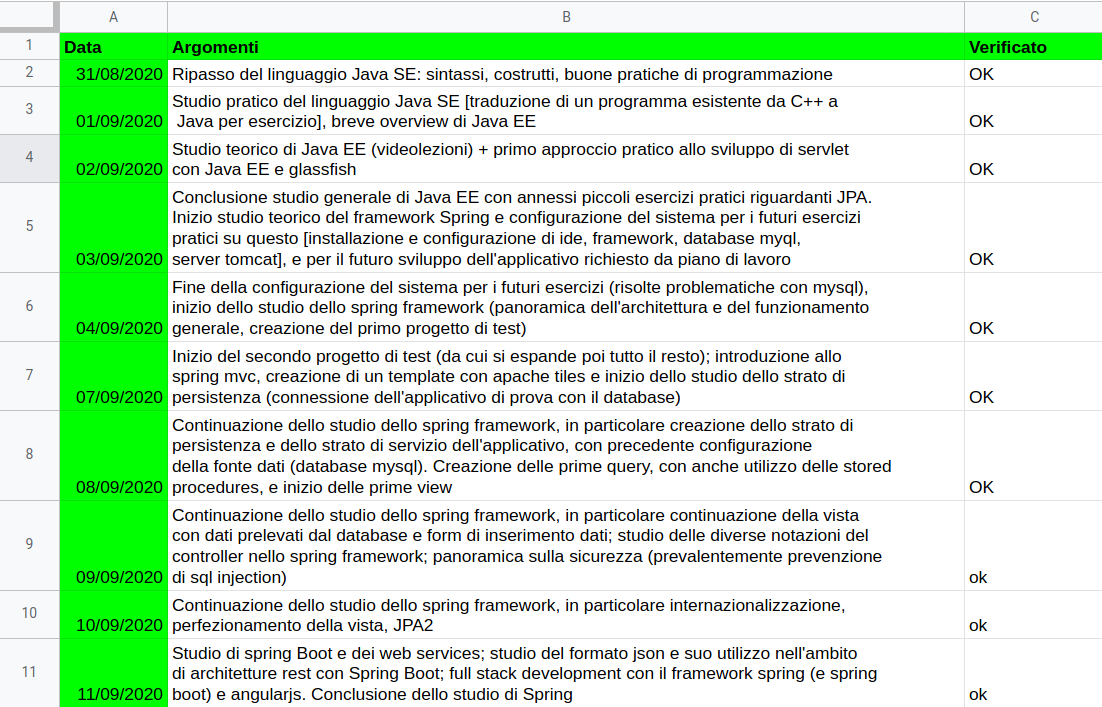
\includegraphics[height=6.5cm]{immagini/drive}
  \captionof{figure}{Porzione del registro delle attività.}
\end{minipage} \\

Per quanto riguarda il salvataggio e il versionamento del codice e della documentazione prodotti, inoltre, ho fatto uso della \textit{repository GitLab} aziendale.

\subsection{Vincoli tecnologici}

Per quanto riguarda i vincoli tecnologici, posso dire di essere stato abbastanza libero nella scelta di quali strumenti utilizzare; i vincoli a cui sono sottostato sono quindi stati decisi principalmente da me, in accordo con il tutor aziendale. Questi sono qui riportati.

\subsubsection*{Sistema operativo}

Essendo il prodotto a cui ho lavorato non coperto da segreto industriale, ho svolto l'intero progetto sulla mia macchina senza bisogno di software esterni per rispettare le norme di sicurezza aziendali. Il sistema operativo che ho utilizzato per lo sviluppo è stato \textit{GNU/Linux}, in particolare la distribuzione \textit{Arch Linux} a 64 bit.

\subsubsection*{PostgreSQL}
Sebbene il mio lavoro non comprendesse l'utilizzo diretto di un \textit{database}, la componente \textit{back-end} dell'applicativo fa uso del \textit{database} relazionale \textit{PostgreSQL}; ho avuto modo di utilizzare questa tecnologia durante il processo di collaudo, per verificare che i dati inseriti dall'applicazione venissero correttamente immagazzinati dal \textit{database}.

\subsubsection*{Docker}
Per effettuare il \textit{deploy} della componente \textit{back-end} dell'applicativo, necessaria al processo di collaudo su dispositivo mobile, ho fatto uso dello strumento di containerizzazione \textit{Docker}. Questo mi ha permesso di rendere la suddetta componente installabile facilmente su qualsiasi sistema.

\subsubsection*{Android Studio}
Per effettuare il collaudo di quanto sviluppato su dispositivo mobile, sono stato vincolato all'ambiente di sviluppo integrato \textit{Android Studio}, fornito gratuitamente dall'azienda \textit{JetBrains}, per la compilazione dell'applicazione per dispositivi \textit{Android}; in accoppiata a questo ho utilizzato il \textit{tool ADB} (\textit{Android Debug Bridge}) per l'installazione dell'applicazione sul dispotivo.

\subsubsection*{Documentazione}
Per quanto riguarda la documentazione, dopo i consigli del mio tutor aziendale la mia scelta è ricaduta sul \textit{tool Compodoc}, uno strumento simile a \textit{Javadoc} per applicazioni sviluppate tramite il \textit{framework Angular}; questo strumento ha permesso la generazione automatica di documentazione a partire da commenti strutturati al codice.

\subsection{Obiettivi}

Insieme al tutor aziendale ho delineato gli obiettivi dello \textit{stage} e li ho riportati in un piano di lavoro validato dal tutor interno, il prof. Tullio Vardanega. \\
Ogni obiettivo possiede un nome formato nel seguente modo:
\begin{center}
  \centering
  \texttt{O-[tipologia][numero]}
\end{center} dove:
\begin{itemize}
  \item \texttt{[tipologia]} indica la tipologia di obiettivo. Questa può essere:
  \begin{itemize}
    \item \texttt{O}: obbligatorio, ossia un obiettivo vincolante e necessario da soddisfare;
    \item \texttt{D}: desiderabile, ossia un obiettivo non vincolante ma dal riconoscibile valore aggiunto;
    \item \texttt{F}: facoltativo, ossia un obiettivo non vincolante e rappresentante un valore aggiunto non competitivo.
  \end{itemize}
  \item \texttt{[numero]} consiste in un numero, progressivo per ogni tipologia.
\end{itemize}

Gli obiettivi inizialmente individuati sono riportati nella seguente tabella.
\newpage

\begin{table}[h]
\begin{tabularx}{\textwidth}{|l|X|}
\hline
\textbf{Obiettivo}           & \textbf{Descrizione}                                                                                                                          \\ \hline
\texttt{O-O1} & Acquisizione delle competenze su linguaggi di programmazione, frameworks e strumenti di supporto                                              \\ \hline
\texttt{O-O2} & Capacità di raggiungere gli obiettivi richiesti in autonomia seguendo il cronoprogramma                                                       \\ \hline
\texttt{O-O3} & Portare a termine le implementazioni previste con una percentuale di superamento pari all'80\%                                                \\ \hline
\texttt{O-D1} & Portare a termine le implementazioni previste con una percentuale di superamento pari al 100\%                                                \\ \hline
\texttt{O-F1} & Dare un contributo importante nelle fasi di progettazione delle maschere con l'obiettivo di realizzare una app usabile, responsive e adaptive \\ \hline
\texttt{O-F2} & Implementare la lettura del QR Code dirattamente dalla fotocamera dello smartphone, evitando quindi inserimenti manuali                       \\ \hline
\end{tabularx}
\caption{Obiettivi di progetto originali.}
\end{table}

In corso di progetto il piano di lavoro è stato rimodulato, in quanto ho svolto parte del lavoro in un tempo minore del previsto; ai precedenti obiettivi si è quindi aggiunto il seguente:

\begin{table}[h]
\begin{tabularx}{\textwidth}{|l|X|}
\hline
\textbf{Obiettivo}           & \textbf{Descrizione}                                                                                                                          \\ \hline
\texttt{O-D2} & Containerizzazione della componente \textit{back-end} del progetto \textit{SyncTrace}                                              \\ \hline
\end{tabularx}
\caption{Ulteriorie obiettivo, aggiunto in corso di progetto.}
\end{table}

Il piano di lavoro identifica inoltre i prodotti attesi; questi sono:
\begin{itemize}
  \item Un \textbf{documento tecnico} che descriva le maschere utilizzate;
  \item Il \textbf{codice} rilasciato sul \textit{repository} indicato dall'azienda.
\end{itemize}

%**************************************************************

\section{Motivazione della scelta}

Sono venuto a conoscenza di Sync Lab durante l'evento \textbf{StageIT 2020}. Questo evento, organizzato dal professor Tullio Vardanega dell'\textit{Università degli Studi di Padova} in collaborazione con l'associazione di imprenditori \textit{Assindustria Venetocentro}, è un'occasione in cui gli studenti di diverse facoltà dell'università di Padova vengono messi in contatto con le aziende presenti sul territorio. \\
L'evento viene organizzato annualmente; quest'anno, però, a causa dell'emergenza sanitaria non si è potuto svolgere in presenza. Nonostante questo, l'adesione da parte delle aziende e degli studenti è stato comunque soddisfacente, anche grazie al fatto che, seguendo gli incontri con le aziende per via telematica, è stato possibile contattarne più di una contemporaneamente. \\

\begin{minipage}{\linewidth}
  \centering
    
\includegraphics[height=1.1cm]{immagini/stageit}
  \captionof{figure}{Logo di \textit{StageIT 2020}.}
  \caption*{\textbf{Fonte:} assindustriavenetocentro.it}
\end{minipage} \\

Durante l'evento \textit{StageIT} ho avuto occasione di parlare con i rappresentanti di quattro aziende operanti nel comune di Padova, tra cui l'ing. Fabio Pallaro di Sync Lab. \\
Gli ambiti di \textit{stage} a cui ero interessato erano principalmente tre: sviluppo software \textit{mobile}, \textit{data science} e \textit{cybersecurity}. Uno dei motivi per cui ho optato per Sync Lab come azienda è stato che l'ing. Pallaro mi ha offerto due diversi ambiti di \textit{stage}: uno riguardante lo sviluppo di un'applicazione per dispositivi mobili tramite \textit{framework Ionic}, e uno riguardante l'aspetto di sicurezza dei prodotti che l'azienda stava e avrebbe sviluppato con altri tirocinanti, entrambi ambiti a cui ero particolarmente interessato. L'azienda, inoltre, mi è sembrata molto attenta agli studenti interessati a un tirocinio presso di essa, segno a mia opinione di serietà, professionalità e apertura a nuove esperienze. \\
Per quanto riguarda il progetto, ho infine optato per lo sviluppo di un applicativo mobile per svariati motivi, anzitutto l'ambito: la tematica del \textit{contact tracing} mi è infatti fin da subito interessata per l'utilità che può avere in situazioni come quella attuale. Oltre a questo, ho trovato che le tecnologie che sarei poi andato ad utilizzare fossero interessanti da un punto di vista personale e, soprattutto, professionale: i linguaggi \textit{JavaScript} e \textit{TypeScript} e i \textit{framework} web e \textit{mobile} come \textit{Angular} e \textit{Ionic}, infatti, sono utilizzati sempre di più frequentemente dalle aziende operanti nel settore \textit{IT}.

%**************************************************************

\section{Formazione}

Ho dedicato il primo mese del mio tirocinio allo studio e all'approfondimento di tutte le conoscenze che mi sarebbero servite, o mi sarebbero state utili, a sviluppare il progetto di \textit{stage} vero e proprio. Gli \textbf{strumenti} che ho utilizzato a tale scopo sono molteplici: anzitutto, ho fatto uso della piattaforma \textit{Udemy} per acquisire le informazioni teoriche riguardanti le tecnologie oggetto di studio; a questo ho associato anche l'utilizzo della piattaforma \textit{YouTube}, sulla quale ho trovato svariati video di particolare utilità. Per quanto riguarda gli esercizi pratici, invece, ho fatto uso sia della piattaforma \textit{Udemy} che di \textit{tool} per l'esercitazione, quali ad esempio il pacchetto \textit{npm "LearnYouNode"} per quanto riguarda lo studio del \textit{runtime NodeJS}. \\

\begin{minipage}{\linewidth}
  \centering
    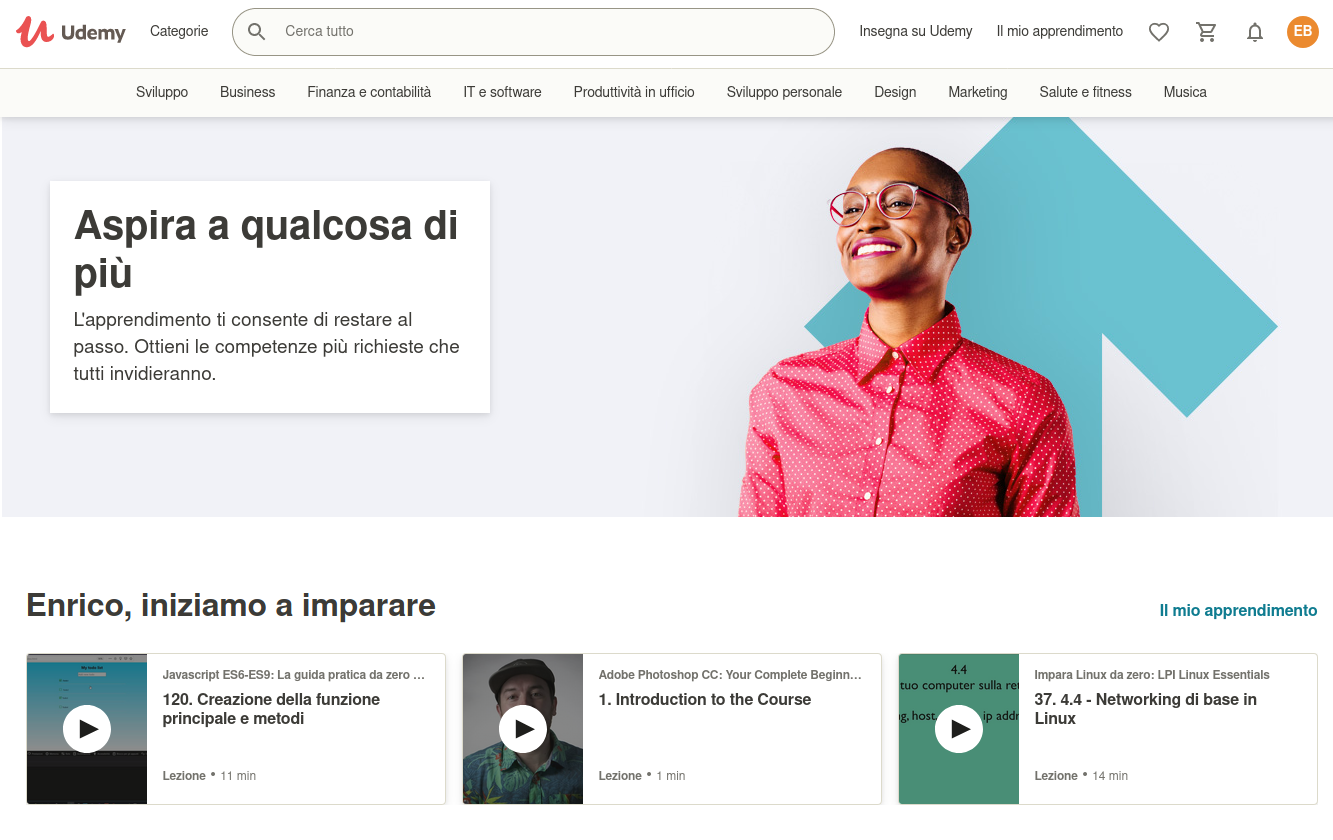
\includegraphics[height=5.5cm]{immagini/udemy}
  \captionof{figure}{\textit{Homepage} della piattaforma \textit{Udemy}.}
  \caption*{\textbf{Fonte:} udemy.com}
\end{minipage}

\subsection{Tecnologie}

In questa sezione sono elencate le tecnologie che ho studiato e appreso; in particolare, ad ogni tecnologia elencata è associata la descrizione del suo utilizzo nell'ambito dello stage. \\
Per quanto riguarda i \textbf{linguaggi di programmazione}, quelli che ho approfondito sono i seguenti:

\begin{itemize}
  \item \textbf{Java}: di questo linguaggio ho studiato principalmente la sintassi, i costrutti di base e, soprattutto, l'implementazione di \textit{servlet} e le \textit{JPA} (\textit{Java Persistence API}) del linguaggio \textit{Java Enterprise Edition}. Sebbene il mio progetto non prevedesse lo sviluppo in codice \textit{Java}, la componente \textit{back-end} del prodotto cui il mio progetto appartiene è scritto con questo linguaggio in accoppiata al \textit{framework Spring}; ho quindi ritenuto opportuno, insieme al tutor aziendale, approfondire questo argomento per poter comprendere almeno a grandi linee il funzionamento del \textit{back-end};
  \item \textbf{JavaScript}: prima di cominciare lo \textit{stage} avevo già delle conoscenze abbastanza radicate di questo linguaggio; di questo ho quindi studiato aspetti avanzati, quali \textit{promises}, \textit{fetch api} e le funzioni asincrone. Sebbene anche questo linguaggio non fosse previsto dal mio progetto, è stato altresì utile da studiare come base per lo studio di \textit{TypeScript};
  \item \textbf{TypeScript}: questo linguaggio è stato quello principalmente utilizzato per lo sviluppo dell'applicativo del mio progetto. Avendo già studiato \textit{JavaScript}, di cui \textit{TypeScript} è un \textit{super-set}, lo studio è stato semplice e veloce.
\end{itemize}

Lo studio di ogni linguaggio di programmazione è stato inoltre associato allo studio di uno o più \textbf{framework}; questi sono:
\begin{itemize}
  \item \textbf{Spring}: di questo \textit{framework}, utilizzato in ambito \textit{Java}, ho studiato a grandi linee il funzionamento generale, comprendente i diversi strati da cui è composto un applicativo sviluppato con questa tecnologia (\textit{database}, persistenza, \textit{business} e presentazione). Come riportato precedentemente, il mio progetto non prevedeva lo sviluppo in codice \textit{Java} ma è stato utile per comprendere il funzionamento della componente \textit{back-end}, e lo stesso vale per il \textit{framework Spring};
  \item \textbf{Angular}: questo \textit{framework}, utilizzato con linguaggio \textit{TypeScript}, è la tecnologia utilizzata per lo sviluppo dell'applicativo di cui il mio progetto prevedeva il \textit{porting}; è stato quindi necessario studiarlo per capire al meglio come fosse strutturato tale applicativo. Oltre a questo, il \textit{framework Ionic}, con il quale ho sviluppato il mio progetto, prevede l'utilizzo di un sottostrato \textit{Angular}; ho quindi usato questo \textit{framework} anche per lo sviluppo in sé;
  \item \textbf{Ionic}: questo \textit{framework}, pensato per lo sviluppo di \textit{PWA} (\textit{Progressive Web Apps}) con codice \textit{TypeScript}, è stato quello più da me utilizzato per lo sviluppo. Ho studiato questo linguaggio tramite la documentazione fornita dall'\textit{Ionic Team}, in quanto a mio parere esaustiva e ben strutturata.
\end{itemize}

Per completare le mie conoscenze in ambito \textit{back-end JavaScript}, inoltre, ho studiato il \textit{runtime} \textbf{NodeJS}. Nessun componente del prodotto a cui il mio progetto appartiene è sviluppato interamente con \textit{NodeJS}; alcune componenti di esso vengono utilizzate, però, per la gestione del collegamento tra la componente \textit{front-end} e quella \textit{back-end} dell'applicativo di cui ho eseguito il \textit{porting}. \\
Ho infine approfondito \textbf{Docker}, piattaforma che automatizza il \textit{deployment} di applicazioni all'interno di macchine virtuali \textit{linux} minimali. Ho approfondito questo argomento a sviluppo già cominciato, poiché per il processo di collaudo si è reso necessario per me avere la componente \textit{back-end} del prodotto su un server accessibile via \textit{http}, e mi è stato proposto di containerizzare tale componente per poter effettuare un \textit{deployment} più efficiente.

\subsection{Progetto}

Come precedentemente riportato, il mio progetto è consistito nell'effettuare il \textit{porting} di una \textit{web application} su dispositivi mobili tramite il \textit{framework Ionic}. L'applicazione web, consistente in una \textit{Single Page Application} sviluppata in \textit{TypeScript} tramite il \textit{framework Angular}, offre le stesse funzionalità dell'applicativo sviluppato da me; molte di queste, però, non sono traslabili direttamente su \textit{mobile}, poiché consistenti di elementi non nativi dei sistemi operativi mobili. Esempio di ciò sono sia piccolezze estetiche, quali ad esempio i bottoni, i \textit{form} e gli \textit{alert}, che l'utilizzo delle risorse hardware del sistema, quali ad esempio la fotocamera, i bottoni fisici e gli strumenti di misura come l'accelerometro. Ho quindi effettuato anche uno studio su quanti e quali componenti software avrei dovuto cambiare per sviluppare correttamente il mio prodotto.

%**************************************************************

% !TEX encoding = UTF-8
% !TEX TS-program = pdflatex
% !TEX root = ../tesi.tex

%**************************************************************
\chapter{Il progetto di stage}
\label{cap:progetto-stage}
%**************************************************************

\section{Analisi dei requisiti}

Sezione contenente l'analisi dei requisiti del prodotto software. In questa sezione verranno riportati anche i diagrammi dei casi d'uso dell'applicativo e, possibilmente, i \textit{mockup} dell'applicazione creati prima di cominciare le attività di progettazione e codifica.

%**************************************************************

\section{Progettazione}

Sezione contenente le scelte progettuali che ho preso, insieme al tutor esterno, per lo sviluppo dell'applicativo. Poiché gran parte delle scelte è stata presa durante il tirocinio antecedente al mio, questa sezione non avrà una grande estensione; nonostante questo, alcune scelte progettuali sono state prese da me, e ritengo quindi giusto riportarle.

%**************************************************************

\section{Codifica}

Sezione contenente una descrizione dell'attività di codifica applicata al mio progetto.

%**************************************************************

\section{Verifica}

Breve introduzione all'attività di verifica svolta, in cui riassumerò le modalità adottate nel caso del mio progetto software e gli strumenti utilizzati per il \textit{testing}.

\subsection{Analisi statica}

Descrizione dell'utilizzo dell'analisi statica per il controllo di conformità del codice agli standard. In questa sottosezione parlerò anche degli strumenti utilizzati per effettuare l'analisi statica del codice e dei risultati ottenuti in quest'ambito.

\subsection{Test di unità}

Sezione riportante tutte le informazioni riguardanti i test di unità implementati e i risultati delle misure.

%**************************************************************

\section{Validazione e collaudo}

Sezione contenente l'analisi delle attività di validazione eseguite. La sezione sarà divisa in due sottosezioni non numerate: la prima riguarderà la validazione, e quindi conterrà l'analisi dei requisiti soddisfatti; la seconda conterrà l'analisi del collaudo. In quest'ultima sottosezione parlerò anche della containerizzazione del back-end di SyncTrace, poiché è stata un'attività fondamentale per poter eseguire il collaudo dell'applicazione su un dispositivo mobile.

%**************************************************************

\section{Risultati ottenuti}

Sezione contenente una visione d'insieme dei risultati ottenuti, ossia un riassunto di quanto sviluppato, verificato, validato e documentato.

% !TEX encoding = UTF-8
% !TEX TS-program = pdflatex
% !TEX root = ../tesi.tex

%**************************************************************
\chapter{Valutazioni retrospettive}
\label{cap:valutazioni-retrospettive}
%**************************************************************

\section{Soddisfacimento degli obiettivi}
Una volta conclusi i processi di sviluppo e documentazione ho analizzato insieme al tutor aziendale gli obiettivi fissati ad inizio \textit{stage}, al fine di individuarne il grado di soddisfacimento e poter effettuare un'analisi a posteriori di cosa avrei potuto gestire meglio. In \hyperref[tab:grado-soddisfacimento]{Tabella 4.1} riporto gli obiettivi fissati, il loro grado di soddisfacimento e una breve nota che sintetizza questo soddisfacimento. \\

\begin{table}[h]
  \label{tab:grado-soddisfacimento}
  \begin{center}
\begin{tabular}{llp{8cm}}
\textbf{Obiettivo}         & \textbf{Risultato}               & \textbf{Note}            \\ \hline
\multicolumn{1}{|l|}{\texttt{O-O1}} & \multicolumn{1}{l|}{Soddisfatto} & \multicolumn{1}{p{8cm}|}{Ho correttamente acquisito le competenze su tutti i linguaggi di programmazione, i \textit{framework} e gli strumenti di supporto previsti dal piano di lavoro} \\ \hline
\multicolumn{1}{|l|}{\texttt{O-O2}} & \multicolumn{1}{l|}{Soddisfatto} & \multicolumn{1}{p{8cm}|}{Ho correttamente seguito il cronoprogramma in autonomia, arrivando a impiegare meno tempo di quanto previsto} \\ \hline
\multicolumn{1}{|l|}{\texttt{O-O3}} & \multicolumn{1}{l|}{Soddisfatto} & \multicolumn{1}{p{8cm}|}{Ho portato a termine le implementazioni previste con una percentuale di superamento pari al 100\%, arrivando a sviluppare anche funzionalità aggiuntive} \\ \hline
\multicolumn{1}{|l|}{\texttt{O-D1}} & \multicolumn{1}{l|}{Soddisfatto} & \multicolumn{1}{p{8cm}|}{Come sopra} \\ \hline
\multicolumn{1}{|l|}{\texttt{O-D2}} & \multicolumn{1}{l|}{Soddisfatto} & \multicolumn{1}{p{8cm}|}{Ho effettuato la corretta containerizzazione della componente \textit{back-end} del progetto \textit{SyncTrace}, rendendo disponibili anche le interfacce grafiche per la gestione dei microservizi da cui è composto e del \textit{database}} \\ \hline
\multicolumn{1}{|l|}{\texttt{O-F1}} & \multicolumn{1}{l|}{Soddisfatto} & \multicolumn{1}{p{8cm}|}{Ho effettuato una corretta progettazione che ha reso l'applicazione sviluppata usabile, \textit{responsive} e \textit{adaptive}} \\ \hline
\multicolumn{1}{|l|}{\texttt{O-F2}} & \multicolumn{1}{l|}{Soddisfatto} & \multicolumn{1}{p{8cm}|}{Ho implementato correttamente la lettura del \textit{QR Code} direttamente della fotocamera. Per ragioni di compatibilità con le scelte di ogni utente, ho inoltre reso disponibile anche l'inserimento manuale del codice} \\ \hline
\end{tabular}
\end{center}
\caption{Grado di soddisfacimento degli obiettivi di \textit{stage}.}
\end{table}

Mi sono inoltre impegnato a consegnare tutti i prodotti richiesti dall'azienda; questi sono riassunti dalla \hyperref[tab:prodotti-sviluppati]{Tabella 4.2}.

\begin{table}[h]
  \label{tab:prodotti-sviluppati}
  \begin{center}
  \begin{tabular}{lp{9cm}}
  \textbf{Prodotto}                        & \textbf{Note}                                                                                                                                                                                                                                                                                                                                    \\ \hline
  \multicolumn{1}{|l|}{Codice}             & \multicolumn{1}{p{9cm}|}{Durante tutto il processo di sviluppo ho utilizzato il repository aziendale riservato agli stage. Ho quindi consegnato ufficialmente il codice effettuando il \textit{merge} dei \textit{branch} da me creati sul \textit{master branch}}                                                                                                               \\ \hline
  \multicolumn{1}{|l|}{Documentazione}     & \multicolumn{1}{p{9cm}|}{La documentazione che ho consegnato consiste nella documentazione tecnica. Questa è integrata nei \textit{file} contenenti il codice, e ho provveduto ad automatizzarne la visualizzazione, con il \textit{tool Compodoc}, tramite la creazione di uno \textit{script npm}}                                                                             \\ \hline
  \multicolumn{1}{|l|}{Containerizzazione} & \multicolumn{1}{p{9cm}|}{Per quanto concerne la containerizzazione, ho rilasciato sul \textit{repository} precedentemente citato due \textit{file yml} che, eseguiti tramite \textit{docker compose}, costruiscono e mettono a disposizione rispettivamente la componente \textit{back-end} di SyncTrace e le interfacce grafiche per la gestione dei microservizi \textit{Spring} e del \textit{database}} \\ \hline
  \end{tabular}
\end{center}
\caption{Prodotti sviluppati e messi a disposizione dell'azienda.}
  \end{table}

In conclusione posso ritenermi soddisfatto di quanto svolto, poiché sono riuscito a completare tutti i prodotti richiesti nel tempo prestabilito e con il massimo grado di soddisfacimento degli obiettivi. \\
Ho riscontrato soltanto due problematiche: una riguardante tutto lo \textit{stage} e una riguardante soltanto l'attività di analisi dei requisiti. La prima è che, purtroppo, ho dovuto svolgere gran parte del mio lavoro in \textit{smart working}, non potendo accedere alla sede per la maggior parte delle giornate lavorative. Per quanto sia comunque riuscito a organizzarmi al meglio per lavorare da casa, infatti, avrei preferito frequentare maggiormente l'azienda, poiché quando mi sono recato di persona ho potuto constatare un clima costruttivo e di collaborazione, a mio parere importante per la mia crescita lavorativa. Naturalmente, questo non è imputabile all'azienda ma al periodo attuale; giudico infatti responsabile questa scelta da parte dell'azienda. \\
La seconda problematica che ho riscontrato riguarda l'analisi dei requisiti. Sebbene il prodotto su cui il mio progetto è basato offrisse una documentazione tecnica estremamente dettagliata e utile allo scopo, parte dell'analisi dei requisiti non è stata caricata sul \textit{repository} aziendale, e questo ha rallentato lievemente la mia attività di analisi dei requisiti. \\
Per quanto concerne gli obiettivi personali posso, anche in questo frangente, dirmi pienamente soddisfatto del percorso che ho svolto. Era infatti mia intenzione approfondire l'ambito dello sviluppo di applicativi \textit{mobile} e utilizzare i linguaggi \textit{JavaScript} e \textit{TypeScript}, in accoppiata ad almeno un \textit{framework} di attuale utilizzo. Dallo \textit{stage} sono riuscito ad ottenere entrambi, poiché ho sviluppato un'applicazione per dispositivi mobili proprio tramite l'utilizzo di \textit{TypeScript} e dei due framework \textit{Angular} e \textit{Ionic}.


%**************************************************************

\section{Bilancio formativo}

\subsection{Maturazione professionale}

Lo \textit{stage} che ho effettuato mi ha portato a sviluppare diverse competenze, sia di natura tecnica che professionale. \\
Per quanto riguarda le \textbf{tecnologie} che ho appreso durante il mio periodo in azienda ci sono anzitutto quelle che riguardano \textit{JavaScript} e tutto ciò che ne deriva: ho infatti approfondito il linguaggio \textit{TypeScript}, arrivando ad averne una conoscenza abbastanza estesa, e  soprattutto ho appreso il funzionamento dei \textit{framework Angular} e \textit{Ionic}. Di questi ultimi due sono arrivato ad avere una conoscenza di buon livello, applicabile anche al mio futuro lavorativo, poiché ho effettuato la codifica del prodotto software in maniera paragonabile allo sviluppo di un applicativo reale e vendibile da un'azienda. \\
Ho inoltre studiato e utilizzato correttamente \textit{Docker}, strumento sempre più utilizzato dalle aziende per la grande scalabilità che offre durante il processo di sviluppo. Ho infine conosciuto, seppur superficialmente, altre tecnologie molto utilizzate odiernamente dalle aziende; tra queste posso citare il linguaggio \textit{Java}, il \textit{framework Spring} e il \textit{database} relazionale \textit{PostgreSQL}. \\
Per quanto riguarda le competenze di \textbf{natura professionale}, ho potuto toccare con mano il funzionamento della metodologia \textit{Agile}, che in Sync Lab si realizza con l'adozione del metodo \textit{Scrum}; anche questo modello di sviluppo è sempre più utilizzato dalle aziende moderne, poiché permette molta flessibilità permettendo al contempo di raggiungere alti livelli di produttività e qualità. \\
Un'ultima competenza che ho acquisito è definibile con il termine, generico ma corretto, \textit{soft skills}; in questo rientrano i rapporti con i colleghi e con i responsabili, l'organizzazione reale del lavoro e la suddivisione dei compiti all'interno dell'azienda.


\subsection{Rapporto tra università e lavoro}

Come ho esposto a inizio documento, lo \textit{stage} è una parte fondamentale del percorso formativo di uno studente; questo periodo, infatti, permette di uscire dagli schemi vissuti durante i precedenti anni di università, potendo toccare con mano la vita lavorativa all'infuori di essa. Lo \textit{stage} e lo studio accademico sono, a mio parere, complementari, poiché uno \textit{stage} non può essere effettuato al meglio senza il percorso formativo accademico che lo precede, e quest'ultimo non può dirsi concluso finché non viene effettuato uno \textit{stage}. \\
Ritengo che la formazione accademica mi sia risultata utile principalmente per la \textit{forma mentis} che mi ha dato; più precisamente, è mia opinione che una componente fondamentale, necessaria allo svolgimento di un tirocinio, sia l'attitudine al lavoro e al rispetto delle tempistiche previste. In questo vedo un'analogia soprattutto con il corso di Ingegneria del Software, più nello specifico con il progetto didattico: ritengo infatti che la conoscenza dei processi e delle attività che portano alla realizzazione di un prodotto software, trattati durante questo corso, sia stata di grande aiuto nel comprendere i meccanismi che un'azienda adotta per portare a compimento il lavoro. \\
Per quanto riguarda la conoscenza delle tecnologie, invece, ho riscontrato una carenza da parte del percorso universitario che ho affrontato; avendo sviluppato un prodotto tramite l'utilizzo di tecnologie pensate per il web, non ho potuto non fare un parallelismo con quanto studiato durante il corso di laurea. Sebbene sia vero che le tecnologie, soprattutto in questo ambito, sono in continua evoluzione e quindi risulta difficile studiarne una che non diventi obsoleta in relativamente poco tempo, ritengo che sarebbe comunque stato utile approfondire lo sviluppo tramite \textit{framework} durante il mio percorso accademico. Nonostante questo, ritengo che effettuare un tirocinio abbia anche lo scopo di apprendere tecnologie all'avanguardia utilizzate dalle aziende; in questo contesto, quindi, si conferma quanto ho precedentemente affermato, e non posso quindi che ritenermi pienamente soddisfatto dell'intero percorso formativo che ho svolto.

%**************************************************************

% \appendix
% % !TEX encoding = UTF-8
% !TEX TS-program = pdflatex
% !TEX root = ../tesi.tex

%**************************************************************
\chapter{Appendice A}
%**************************************************************

% \epigraph{Citazione}{Autore della citazione}
             % Appendice A

%**************************************************************
% Materiale finale
%**************************************************************
% \backmatter
% \printglossaries
% % !TEX encoding = UTF-8
% !TEX TS-program = pdflatex
% !TEX root = ../tesi.tex

%**************************************************************
% Bibliografia
%**************************************************************

\cleardoublepage
\chapter{Bibliografia}

% \nocite{*}
% % Stampa i riferimenti bibliografici
% \printbibliography[heading=subbibliography,title={Riferimenti bibliografici},type=book]

% Stampa i siti web consultati
\printbibliography[heading=subbibliography,title={Siti web consultati},type=online]

\end{document}
